\documentclass[twocolumn]{article}
\usepackage{arxiv}
\usepackage[utf8]{inputenc}
\usepackage[T1]{fontenc}
\usepackage{hyperref}
\usepackage{url}
\usepackage{booktabs}
\usepackage{amsfonts}
\usepackage{amsmath}
\usepackage{nicefrac}
\usepackage{microtype}
\usepackage{graphicx}
\usepackage{natbib}
\usepackage{doi}
\graphicspath{{figures/}}
% relax float placement so full-width figures distribute instead of piling up at the end
\setcounter{topnumber}{3}\setcounter{totalnumber}{4}
\renewcommand{\topfraction}{0.92}\renewcommand{\textfraction}{0.06}\renewcommand{\floatpagefraction}{0.78}
\renewcommand{\dbltopfraction}{0.92}\renewcommand{\dblfloatpagefraction}{0.78}

\title{Internal Excellence, External Collapse: An Audit and Diagnosis of a\\ Knowledge-Distilled Cervical Cytology Classifier Across Datasets}
\renewcommand{\shorttitle}{Internal Excellence, External Collapse}
\author{Cervical Cytology Pipeline}
\hypersetup{pdftitle={Internal Excellence, External Collapse},
pdfsubject={q-bio.QM, cs.CV},
pdfkeywords={cervical cytology, knowledge distillation, domain shift, calibration, SIPaKMeD}}

\begin{document}

\twocolumn[
\begin{@twocolumnfalse}
\maketitle
\begin{abstract}
Automated cervical-cytology screening is increasingly framed as an image-classification problem, and deep convolutional networks now report near-ceiling accuracy on curated single-dataset benchmarks. Whether such accuracy reflects transferable diagnostic competence or merely fits the idiosyncrasies of one slide-preparation protocol remains largely unaudited. We present a rigorous, leakage-aware audit of a knowledge-distilled cervical-cytology classifier. An EfficientNet-B4 teacher (18.5\,M parameters) was trained on the five SIPaKMeD cytomorphology classes with weighted cross-entropy and two-stage fine-tuning, and its knowledge was distilled into an EfficientNet-B0 student (4.67\,M parameters) using the Hinton objective \citep{hinton2015distilling}. In-distribution, the distilled student surpasses its teacher on every metric, reaching accuracy 0.966, balanced accuracy 0.968, macro-F1 0.967, Cohen's $\kappa$ 0.958, one-vs-rest macro AUROC 0.998, and an Expected Calibration Error of 0.015; Grad-CAM \citep{selvaraju2017gradcam} confirms that decisions localize to the nucleus and cell body rather than background. We then evaluate the same student, without retraining, on three external Papanicolaou datasets---Herlev, APACC, and HiCervix---under a deterministic, documented binary Normal-versus-Abnormal label alignment with reported excluded fractions. Cross-dataset accuracy collapses to 0.639 (Herlev), 0.605 (HiCervix), and 0.532 (APACC), falling below the majority-class baseline on two of three datasets despite all AUROC exceeding chance. A diagnostic analysis attributes this collapse not to label-mapping artefacts---class-conditional $P(\text{abnormal})$ separation is positive everywhere and every AUROC $>0.5$---but to operating-point miscalibration that does not transfer across domains and to increasing slide-preparation distance from SIPaKMeD's conventional smear. We further show that the internal accuracy is itself optimistic, inflated by same-field-of-view leakage in the per-cell split. The study contributes a reproducible cross-dataset audit methodology, evidence that distillation can yield a smaller-yet-stronger in-distribution model that nonetheless fails out-of-distribution, and concrete, evidence-led remedies for trustworthy cervical-screening deployment.
\end{abstract}
\keywords{cervical cytology \and knowledge distillation \and domain shift \and calibration \and explainability \and SIPaKMeD}
\bigskip
\end{@twocolumnfalse}
]

\section{Introduction}

Cervical cancer remains one of the most preventable malignancies, and its prevention hinges on the cytological screening of Papanicolaou-stained smears. Because expert cytologists are scarce and manual reading is laborious and subject to inter-observer variability, automated classification of cervical cells has become an active research frontier. Modern deep convolutional networks routinely report accuracies above 0.95 on public benchmarks such as SIPaKMeD \citep{plissiti2018sipakmed}, and this success has fuelled optimism that screening can be partially automated. Yet the dominant evaluation paradigm in this literature is single-dataset: a model is trained and tested on splits drawn from one collection, prepared under one staining and segmentation protocol, and the resulting accuracy is reported as if it were an intrinsic property of the model. This conflates two very different questions---how well a model fits the statistics of a particular slide-preparation pipeline, and how well it would actually generalize to the heterogeneous slides encountered in clinical practice. The gap between these questions is precisely where deployable, trustworthy screening tools succeed or fail, and it is rarely measured.

This paper subjects a representative high-accuracy system to exactly such a measurement. We study a knowledge-distilled classifier in which an EfficientNet-B4 teacher \citep{tan2019efficientnet}, ImageNet-pretrained \citep{deng2009imagenet} and trained on the five SIPaKMeD cytomorphology classes, is distilled into a compact EfficientNet-B0 student through the temperature-scaled Hinton objective \citep{hinton2015distilling}. The student is attractive for deployment because it carries only 4.67\,M parameters against the teacher's 18.5\,M, and we ask whether such compression sacrifices accuracy, calibration, explainability, or generalization. We evaluate the model both within SIPaKMeD and, crucially, across three independent external Papanicolaou datasets---Herlev \citep{jantzen2005herlev}, APACC, and HiCervix \citep{cai2024hicervix}---which differ in staining, segmentation, and slide preparation (conventional smear, auto-segmented crops, and liquid-based cytology). Because the five SIPaKMeD morphology classes do not share a label space with the dysplasia and Bethesda \citep{nayar2015bethesda} schemes of the external datasets, we align them at the only common, deterministically mappable level: a binary Normal-versus-Abnormal decision, with glandular and out-of-scope categories explicitly excluded and the excluded fraction reported as an honesty metric.

Our investigation is organized around four research questions and their hypotheses. \textbf{RQ1}: Can a knowledge-distilled B0 student match the B4 teacher's in-distribution accuracy at a fraction of the parameters? \textbf{H1}: yes, and the regularizing effect of distillation may let the student match or even exceed the teacher. \textbf{RQ2}: Does strong in-distribution accuracy translate to cross-dataset generalization on independent Pap datasets? \textbf{H2}: no---a large internal-to-external gap is expected. \textbf{RQ3}: Is any cross-dataset failure a label-mapping artefact or a genuine model and domain failure? \textbf{H3}: it is genuine domain shift compounded by miscalibration, not a labelling error. \textbf{RQ4}: Do calibration and explainability hold, and does calibration transfer out-of-distribution? \textbf{H4}: in-distribution the model is well-calibrated \citep{guo2017calibration} and its Grad-CAM attributions are plausible, but calibration does not transfer across domains. Together these questions move the evaluation beyond a single accuracy figure toward an account of where, and why, a high-performing model breaks.

In answering them, this work makes the following contributions.

\begin{itemize}
\item A reproducible, leakage-aware cross-dataset audit of a distilled cervical-cytology model across three external Papanicolaou datasets (Herlev, APACC, HiCervix) under a deterministic, documented binary label alignment with reported excluded fractions.
\item A diagnostic methodology that separates labelling artefacts from genuine domain failure, combining class-conditional $P(\text{abnormal})$ separation, an AUROC-above-chance test, and an accuracy-versus-majority-baseline and oracle-threshold analysis.
\item Empirical evidence that the distilled student surpasses its teacher while remaining well-calibrated and explainable in-distribution, yet collapses out-of-distribution, with the collapse attributed to operating-point miscalibration and slide-preparation distance rather than to relabelling \citep{geirhos2020shortcut}.
\item Concrete, evidence-led remedies: leakage-safe cluster-grouped evaluation, stain and domain normalization \citep{macenko2009stain}, per-domain calibration, and the reporting of threshold-free AUROC alongside the excluded fraction.
\end{itemize}

\section{Related Work}

\subsection{Deep Learning for Cervical Cytology}
Automated cervical-cytology screening has been propelled by curated benchmarks, most prominently the SIPaKMeD database of Papanicolaou-stained conventional-smear cells annotated into five cytomorphological classes \citep{plissiti2018sipakmed}, and the earlier Herlev collection of single cells labelled under the WHO dysplasia schema \citep{jantzen2005herlev}. A large body of work reports near-ceiling within-dataset accuracy on these corpora using deep convolutional backbones, and recent liquid-based resources such as HiCervix extend the task to hierarchical Bethesda categories at substantially greater scale \citep{cai2024hicervix,nayar2015bethesda}. Convolutional architectures of the EfficientNet family \citep{tan2019efficientnet}, typically initialised from ImageNet pre-training \citep{deng2009imagenet}, have become a standard high-accuracy, parameter-efficient choice for this domain. However, the overwhelming majority of these studies evaluate on a held-out split of the same database on which they were trained, leaving open the question of whether the reported performance reflects transferable cytological competence or dataset-specific regularities.

\subsection{Knowledge Distillation for Efficient Medical Models}
The deployment of cytology classifiers on resource-constrained or point-of-care hardware motivates model compression, and knowledge distillation \citep{hinton2015distilling} has emerged as a leading strategy: a compact student is trained to match the temperature-softened logits of a larger teacher, frequently recovering---and occasionally exceeding---teacher accuracy through the regularising effect of soft targets. While distillation is now common across medical-imaging tasks, its interaction with out-of-distribution behaviour is rarely examined; a smaller, better-regularised student may generalise no better than its teacher if both have learned the same dataset-specific shortcuts.

\subsection{Generalization, Shortcut Learning, Calibration, and Explainability}
A recurring finding across medical imaging is that high in-distribution accuracy degrades sharply under cross-dataset evaluation, a phenomenon attributable in large part to shortcut learning, whereby networks exploit spurious correlations---staining, scanner, and preparation cues---rather than the intended morphology \citep{geirhos2020shortcut}. Two complementary tools are routinely invoked to interrogate such models. Confidence calibration, quantified by the Expected Calibration Error and reliability diagrams \citep{guo2017calibration}, assesses whether predicted probabilities are trustworthy, yet calibration established in-distribution is seldom verified to transfer across domains. Post-hoc attribution methods such as Grad-CAM \citep{selvaraju2017gradcam} localise the image regions driving a decision and are widely used to argue for clinical plausibility, although they reveal where a model attends rather than whether its reasoning is faithful.

\subsection{The Gap: Standardised Cross-Dataset Label Alignment}
Cross-dataset benchmarking in cervical cytology is further obstructed by incompatible taxonomies: the five SIPaKMeD morphology classes, the seven-grade Herlev dysplasia scheme, and the hierarchical Bethesda system of HiCervix and APACC do not share a common label space, and the requisite projection is frequently one-to-many or undefined \citep{nayar2015bethesda}. Prior comparisons rarely document the mapping or report the fraction of cases excluded because they have no valid correspondence (for instance, glandular lesions with no squamous home), which undermines reproducibility. Our work addresses this gap with a deterministic, fully documented binary Normal-versus-Abnormal alignment and an honesty metric quantifying the excluded fraction, enabling a leakage-aware audit of distilled-model generalisation across three independent Pap datasets.


\begin{table*}[t]
\caption{Datasets used in this study. SIPaKMeD is the sole training source; the other three are
held-out external evaluation sets spanning different slide preparations and label taxonomies.}
\label{tab:datasets}
\centering\small
\begin{tabular}{lllll}
\toprule
Dataset & Role & Preparation / type & Native label space & Size \\
\midrule
SIPaKMeD \citep{plissiti2018sipakmed} & Train (+val) & Conventional smear; cells + FoV & 5 cytomorphology classes & 5{,}015 imgs (4{,}049 cells) \\
Herlev \citep{jantzen2005herlev}      & External eval & Conventional smear; single cells & 7 WHO-dysplasia classes & 917 cells \\
APACC                                  & External eval & Auto-segmented single-cell crops & 4 coarse (healthy/unhealthy/$\dots$) & 1{,}125 cells \\
HiCervix \citep{cai2024hicervix}       & External eval & Liquid-based cytology (LBC) & Hierarchical Bethesda & 4{,}823 cells (8{,}051 total) \\
\bottomrule
\end{tabular}
\end{table*}

\section{Materials}

This study draws on four publicly available cervical-cytology datasets: one for model development and three reserved exclusively for external evaluation. Table~\ref{tab:datasets} summarizes their composition, native label taxonomies, imaging granularity, and slide-preparation characteristics. A defining feature of this collection is that no two datasets share a common annotation schema; this taxonomic heterogeneity is the central obstacle that motivates the deterministic label-alignment procedure described later.

\subsection{Training dataset: SIPaKMeD}

Model training relies on the SIPaKMeD dataset \citep{plissiti2018sipakmed}, comprising 5{,}015 Papanicolaou-stained images acquired from conventional cervical smears. The corpus combines two levels of granularity: 4{,}049 cropped single-cell images and 966 cluster field-of-view (FoV) images. Every image is annotated into one of five cytomorphology classes that describe cell appearance rather than dysplasia grade: Superficial-Intermediate (957), Parabasal (895), Metaplastic (1{,}064), Koilocytotic (1{,}063), and Dyskeratotic (1{,}036). The resulting class distribution is only mildly imbalanced, with a maximum-to-minimum ratio of 1.19. The imagery is markedly heterogeneous in scale, spanning 62--2048 px in width (mean 614.7) and 62--1536 px in height (mean 485.4), reflecting both the dual cell-versus-cluster granularity and variation in acquisition. Critically, the five SIPaKMeD categories form a morphology-based taxonomy with no native notion of normal versus abnormal, which must be reconstructed for any cross-dataset comparison.

\subsection{External evaluation datasets}

To probe generalization beyond the training distribution, we evaluate on three independent datasets, each with its own taxonomy, preparation, and segmentation pipeline.

The Herlev dataset \citep{jantzen2005herlev} contains 917 single-cell images drawn from conventional Papanicolaou smears and labelled under a seven-class WHO-dysplasia scheme: normal\_superficiel, normal\_intermediate, normal\_columnar, light\_dysplastic, moderate\_dysplastic, severe\_dysplastic, and carcinoma\_in\_situ. Each cell is distributed alongside a companion segmentation mask (the {-d.bmp} files), which we discard so that evaluation operates on the raw cell image alone. Of the three external sources, Herlev is the closest to SIPaKMeD in stain and preparation, both being conventional smears.

The APACC dataset provides 1{,}125 automatically segmented single-cell crops in its test split, annotated under a coarse four-category native taxonomy (healthy, unhealthy, rubbish, and bothcells). The two non-cellular categories, rubbish and bothcells, are excluded, leaving a healthy-versus-unhealthy partition. Because its crops are produced by automatic segmentation rather than expert delineation, APACC carries the greatest preparation distance from SIPaKMeD and the noisiest cell-level inputs.

The HiCervix dataset \citep{cai2024hicervix} represents a liquid-based cytology (LBC) source and contributes a test split of 8{,}051 single cells carrying hierarchical Bethesda-system labels \citep{nayar2015bethesda}. We retain the level-1 categories negative and ASC (4{,}823 cells) and exclude the glandular AGC and microbe categories (3{,}228 cells), since glandular lesions have no squamous counterpart in the five-class morphology space; this excluded fraction is reported explicitly as a measure of evaluation honesty.

Taken together, these datasets span morphology-based, WHO-dysplasia, coarse healthy/unhealthy, and Bethesda annotation systems across conventional-smear, liquid-based, and auto-segmented preparations. No single label projection maps these schemes onto one another, which establishes the need for the shared binary normal/abnormal alignment developed in the following section.


\begin{figure*}[t]
\centering
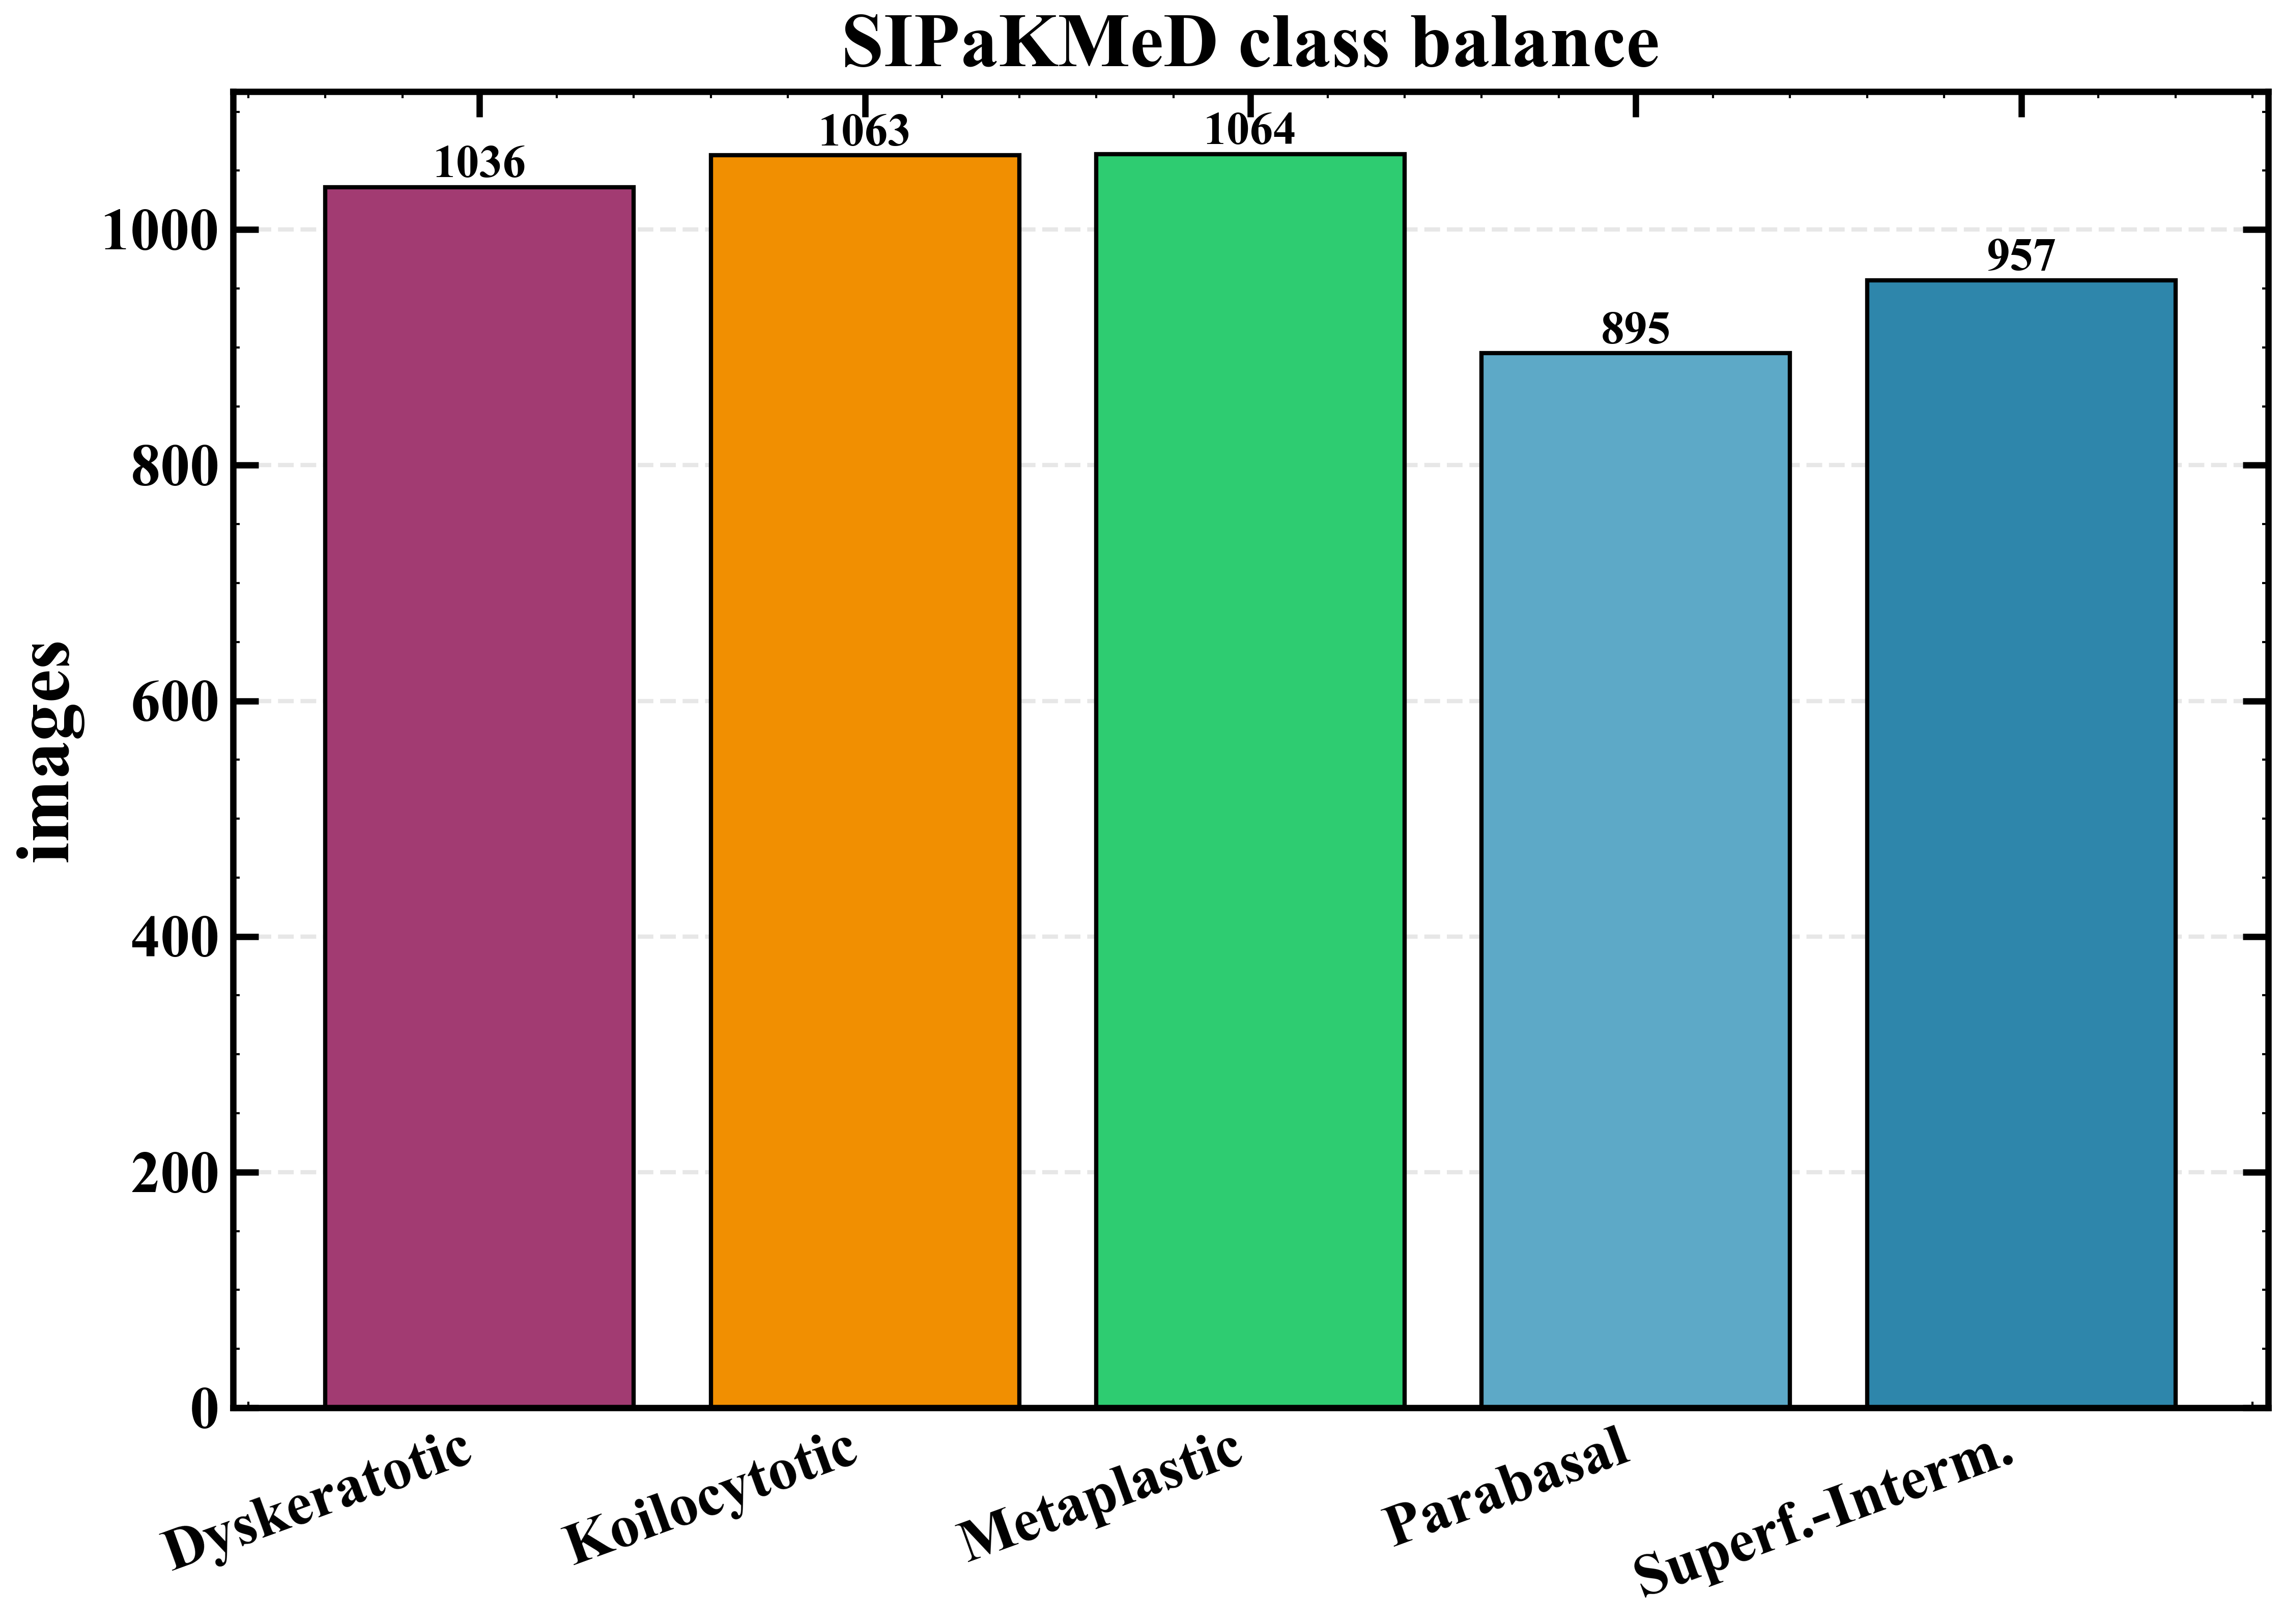
\includegraphics[width=0.40\textwidth]{eda_class_balance.png}\hfill
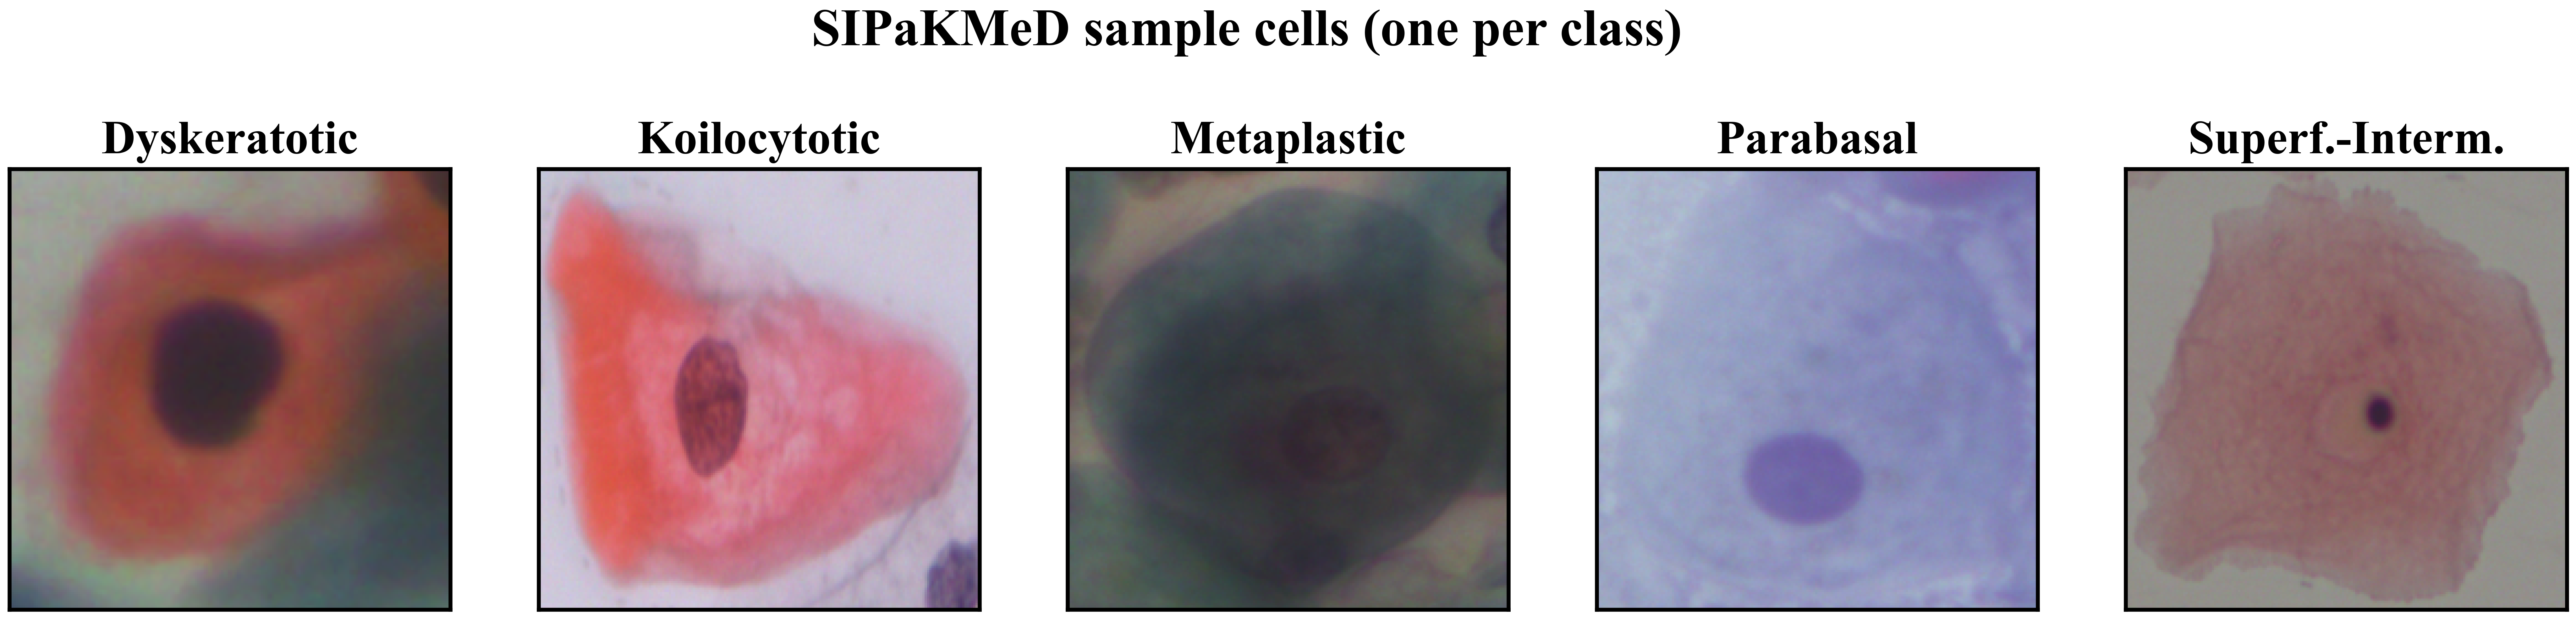
\includegraphics[width=0.56\textwidth]{eda_sample_cells.png}
\caption{Exploratory data analysis of SIPaKMeD. Left: per-class image counts (mild imbalance, ratio $1.19$). Right: representative cells across the five classes.}
\label{fig:eda}
\end{figure*}

I'll write the assigned LaTeX section using only the shared facts provided.

`\section{Exploratory Data Analysis and Data Pipeline}`
`\label{sec:methods_data}`

`\subsection{Exploratory data analysis}`
The training corpus is SIPaKMeD~`\citep{plissiti2018sipakmed}`, a collection of 5{,}015 Papanicolaou-stained conventional-smear images annotated into five cytomorphology classes: Superficial--Intermediate, Parabasal, Metaplastic, Koilocytotic, and Dyskeratotic. Three properties of this corpus shape the entire downstream pipeline, and we summarize them visually in Figure~`\ref{fig:eda}`.

First, the class distribution is only mildly imbalanced. The per-class counts---Dyskeratotic 1{,}036, Koilocytotic 1{,}063, Metaplastic 1{,}064, Parabasal 895, and Superficial--Intermediate 957---yield a majority-to-minority ratio of 1.19. This near-uniform support means that the dominant modelling challenge is morphological discriminability among adjacent cytological categories rather than gross frequency skew; nevertheless, we retain a class-weighted training objective (Section on training) as a conservative safeguard against the residual imbalance.

Second, the imagery is strongly heterogeneous in spatial extent. Image widths span 62--2{,}048~px (mean 614.7) and heights span 62--1{,}536~px (mean 485.4), a roughly thirty-fold range in each dimension. Such variability precludes feeding native resolutions to a convolutional backbone and motivates an explicit, fixed-size resizing stage that places every sample on a common geometric footing.

Third, the dataset exhibits a dual granularity: 4{,}049 of the images are tightly cropped single cells, while the remaining 966 are cluster field-of-view (FoV) images containing multiple overlapping cells. This mixture is biologically faithful---routine smears contain both isolated cells and dense clusters---but it has an important methodological consequence. Cells originating from the same FoV are visually correlated, so a naive per-image split can place near-duplicate views on both sides of a train/validation partition. We flag this here because it directly conditions our later interpretation of the optimistic internal accuracy.

`\subsection{Preprocessing}`
All images pass through a single deterministic preprocessing chain at both training and evaluation time. Each file is decoded and converted to three-channel RGB, then resized to $380\times380$~px, the native input resolution of EfficientNet-B4~`\citep{tan2019efficientnet}`. Crucially, we adopt this same $380\times380$ geometry for \emph{both} the B4 teacher and the B0 student, so that distillation transfers knowledge between networks that observe pixel-identical inputs and the student is never disadvantaged by a resolution mismatch. Pixel intensities are finally standardized with the ImageNet channel statistics---means $(0.485, 0.456, 0.406)$ and standard deviations $(0.229, 0.224, 0.225)$---consistent with the ImageNet-pretrained weights~`\citep{deng2009imagenet}` that initialize both backbones. Fixing resolution and normalization across teacher, student, and all four datasets ensures that any cross-dataset performance gap reflects genuine domain shift rather than incidental differences in the input pipeline.

`\subsection{Data augmentation}`
Stochastic augmentation is applied \emph{exclusively} during training; the validation and all external evaluations use only the deterministic resize-and-normalize chain above, so that reported generalization is never inflated by test-time perturbation. The training-time transforms are deliberately restricted to operations that preserve cytological meaning. We apply random horizontal and vertical flips (each with probability 0.5), random rotation within $\pm72^{\circ}$, and a random affine scaling (zoom) between $0.9$ and $1.1$. These choices exploit a defining symmetry of cytology: a cell has no canonical orientation on the slide, so reflections and rotations generate label-preserving views that encourage rotation- and flip-invariant features rather than memorized pose. The modest scaling band emulates benign variation in cell size and magnification without distorting the nucleus-to-cytoplasm relationships that underpin the diagnostic classes. We deliberately omit colour, contrast, and elastic distortions, which could corrupt the Papanicolaou staining cues and chromatin texture that the classes depend on. This augmentation regime enlarges the effective sample diversity while keeping every synthetic view cytologically plausible.

\section{Model and Training}

\subsection{Architecture}
Both networks in our teacher--student pair are drawn from the EfficientNet family \citep{tan2019efficientnet}, which couples compound width/depth/resolution scaling with mobile inverted-bottleneck blocks to obtain a favourable accuracy-to-parameter trade-off. The teacher is an EfficientNet-B4 ($18.5$\,M parameters) and the student a substantially leaner EfficientNet-B0 ($4.67$\,M parameters), so that distillation operates across roughly a fourfold compression in capacity. Both backbones are initialised from ImageNet-pretrained weights \citep{deng2009imagenet} provided by \texttt{torchvision}; transferring these features is essential given the modest size of SIPaKMeD relative to the data appetite of training such convolutional backbones from scratch. To match the two models within a single preprocessing pipeline, every image---for both teacher and student---is decoded to RGB, resized to the $380\times380$ resolution native to B4, and normalised with the standard ImageNet channel statistics.

We replace the original classifier of each backbone with an identical task head, attached to the pooled backbone features: a one-dimensional batch normalisation layer, a fully connected projection to $512$ units, a ReLU non-linearity, dropout for regularisation, and a final linear layer mapping to the five SIPaKMeD cytomorphology classes. Sharing the head design between teacher and student keeps the logit geometry comparable, which is desirable because distillation aligns the student's softened logits with the teacher's.

\subsection{Two-stage teacher training and knowledge distillation}
The teacher is trained in two stages with the Adam optimiser under a weighted cross-entropy objective, monitoring validation loss for early stopping. Because the five classes are only mildly imbalanced (imbalance ratio $1.19$), we nonetheless apply inverse-frequency class weights, $w_c = N / (K\,n_c)$, where $N$ is the training-set size, $K=5$, and $n_c$ the count of class $c$, so that no minority class is systematically discounted. In the first stage the backbone is frozen and only the new head is optimised at a learning rate of $10^{-3}$ for up to $30$ epochs (early-stopping patience $8$), with a \texttt{ReduceLROnPlateau} schedule (factor $0.3$, patience $4$, minimum learning rate $10^{-6}$); this adapts the randomly initialised head to the pretrained features before any backbone weights are disturbed. In the second stage the entire network is unfrozen and fine-tuned end-to-end at a much smaller learning rate of $10^{-5}$ for up to $50$ epochs (patience $6$), allowing the deep representation to specialise to cervical cytology without erasing the transferred ImageNet structure.

The student is then trained by knowledge distillation \citep{hinton2015distilling} with Adam (learning rate $5\times10^{-5}$, up to $40$ epochs, patience $8$, monitoring validation accuracy). Writing $z_s$ and $z_t$ for the student and (frozen) teacher logits, $y$ for the ground-truth label, $T$ for the temperature and $\alpha$ for the hard-target weight, the loss is
\begin{equation}
\mathcal{L} = \alpha\,\mathrm{CE}\!\left(y, z_s\right) + (1-\alpha)\,T^{2}\,\mathrm{KL}\!\left(\mathrm{softmax}\!\left(z_t/T\right)\,\big\|\,\mathrm{softmax}\!\left(z_s/T\right)\right),
\end{equation}
where the $T^{2}$ factor restores the gradient scale of the softened distillation term. We use $T=4$ and $\alpha=0.1$, placing most of the weight on the teacher's softened class posteriors so that the student inherits the teacher's inter-class similarity structure rather than only the hard labels. All training is performed in PyTorch on a single RTX~5060~Ti GPU with BF16 autocast mixed precision, batch size $32$, and a fixed seed of $42$ over a per-class-stratified $80/20$ train/validation split ($4{,}012$ training and $1{,}003$ validation images).

In practice the teacher early-stopped after $71$ epochs ($30$ frozen plus $41$ fine-tuning) at a final validation accuracy of $0.9442$, while the distilled student early-stopped after $34$ epochs at $0.9661$. The training and validation curves (Figure~\ref{fig:curves}) track closely throughout and show no divergence indicative of overfitting, and the distillation regularisation yields a student whose validation accuracy in fact exceeds that of its larger teacher.


\begin{table*}[t]
\caption{Deterministic binary (Normal/Abnormal) label crosswalk. The model-side decision uses
$P(\mathrm{abnormal})=\sigma(z)_{\mathrm{Koilo}}+\sigma(z)_{\mathrm{Dysk}}$. Glandular and
out-of-scope native categories have no squamous home in the five-class space and are excluded; the
excluded fraction is reported per dataset.}
\label{tab:mapping}
\centering\small
\begin{tabular}{lll}
\toprule
Source & $\rightarrow$ Normal & $\rightarrow$ Abnormal \quad(/ Excluded) \\
\midrule
SIPaKMeD (model) & Superficial-Interm., Parabasal, Metaplastic & Koilocytotic, Dyskeratotic \\
Herlev & superficiel, intermediate, columnar & light/moderate/severe dyspl., carcinoma-in-situ \\
APACC & healthy & unhealthy \quad(rubbish, bothcells excl.) \\
HiCervix & \texttt{level\_1}=negative & \texttt{level\_1}=ASC \quad(AGC, microbe excl.) \\
\bottomrule
\end{tabular}
\end{table*}

I'll write the assigned section. This is a self-contained writing task using the shared facts provided.

\section{Cross-dataset Label Alignment and Evaluation Protocol}

\subsection{Binary label alignment}

The five SIPaKMeD training classes encode squamous cytomorphology (Superficial-Intermediate, Parabasal, Metaplastic, Koilocytotic, Dyskeratotic), whereas the external datasets are annotated under fundamentally different schemes: Herlev follows a seven-tier WHO dysplasia grading, while HiCervix adopts the hierarchical Bethesda terminology \citep{nayar2015bethesda}. These taxonomies do not share a label space with the SIPaKMeD morphology classes. Any attempt to project one onto the other at full granularity is either one-to-many or undefined---a single dysplasia grade spans several morphological appearances, and several morphology classes have no unique Bethesda counterpart. The only level at which all four datasets admit a deterministic, many-to-one mapping is the binary distinction between normal and abnormal cervical cytology. We therefore evaluate cross-dataset performance exclusively in this binary regime, which preserves clinical meaning while avoiding spurious correspondences.

On the model side, we collapse the five-way softmax into a single abnormality score by summing the posterior mass assigned to the two atypical classes,
\begin{equation}
P(\text{abnormal}) = \mathrm{softmax}(z)_{\text{Koilocytotic}} + \mathrm{softmax}(z)_{\text{Dyskeratotic}},
\end{equation}
where $z$ denotes the student logits; the remaining three classes (Superficial-Intermediate, Parabasal, Metaplastic) constitute the normal pool. A cell is called abnormal when $P(\text{abnormal}) \geq \tau$ with a fixed operating point $\tau = 0.5$. On the label side, the per-dataset crosswalk (Table~\ref{tab:mapping}) is fixed in advance and applied without exception. For Herlev, the superficial, intermediate, and columnar normal categories map to Normal, while light, moderate, and severe dysplasia together with carcinoma \emph{in situ} map to Abnormal. For APACC, \emph{healthy} maps to Normal and \emph{unhealthy} to Abnormal. For HiCervix, the level-1 \emph{negative} label maps to Normal and \emph{ASC} to Abnormal.

A deliberate consequence of training on a purely squamous morphology vocabulary is that glandular lesions have no admissible home in the five-class space. Accordingly, Herlev's columnar cells are treated as normal squamous-equivalent only with caution, and the HiCervix glandular (AGC) and microbe categories are excluded outright, as is the case for APACC \emph{rubbish} and \emph{bothcells}. Rather than silently dropping these instances, we report the excluded fraction for each dataset as an explicit honesty metric, so that the denominator underlying every cross-dataset number is transparent.

\subsection{Evaluation metrics}

In-distribution performance on the held-out SIPaKMeD validation split is assessed at full five-class granularity using accuracy, balanced accuracy, macro-averaged F1, Cohen's $\kappa$, and the one-vs-rest macro AUROC, complemented by per-class precision, recall, and F1 and the full $5\times5$ confusion matrix. Probabilistic reliability is quantified with the Expected Calibration Error computed over fifteen equal-width confidence bins, alongside a reliability diagram \citep{guo2017calibration}; the ECE summarizes the average gap between predicted confidence and empirical accuracy and thus probes whether the network's probabilities can be trusted as operating points.

Cross-dataset performance is reported in the binary Normal-versus-Abnormal regime using accuracy, balanced accuracy, sensitivity (recall on the abnormal class), specificity (recall on the normal class), and the threshold-free AUROC computed directly on $P(\text{abnormal})$, together with the binary confusion matrix and the aforementioned excluded fraction. Reporting AUROC separately from the fixed-$\tau$ accuracy is essential: it isolates the model's intrinsic ranking ability from any miscalibration of the decision boundary, allowing us to distinguish a genuine loss of discriminative signal from a mere shift of the optimal operating point across domains.

\subsection{Explainability}

To verify that in-distribution decisions rest on cytologically plausible evidence rather than background artefacts, we apply Grad-CAM \citep{selvaraju2017gradcam} to the student's final convolutional block, gradient-weighting the activation maps with respect to the predicted class to obtain a coarse localization heatmap for one representative cell per class. We emphasize the methodological caveat that Grad-CAM is an attribution technique: it reveals \emph{where} the network attends, not \emph{why} it decides, and spatial coincidence with the nucleus or cytoplasm is evidence of plausible feature use rather than proof of clinically faithful reasoning. We therefore treat the saliency maps as corroborating, not confirmatory, and report them as a transparency aid alongside the quantitative results.


\begin{figure*}[t]
\centering
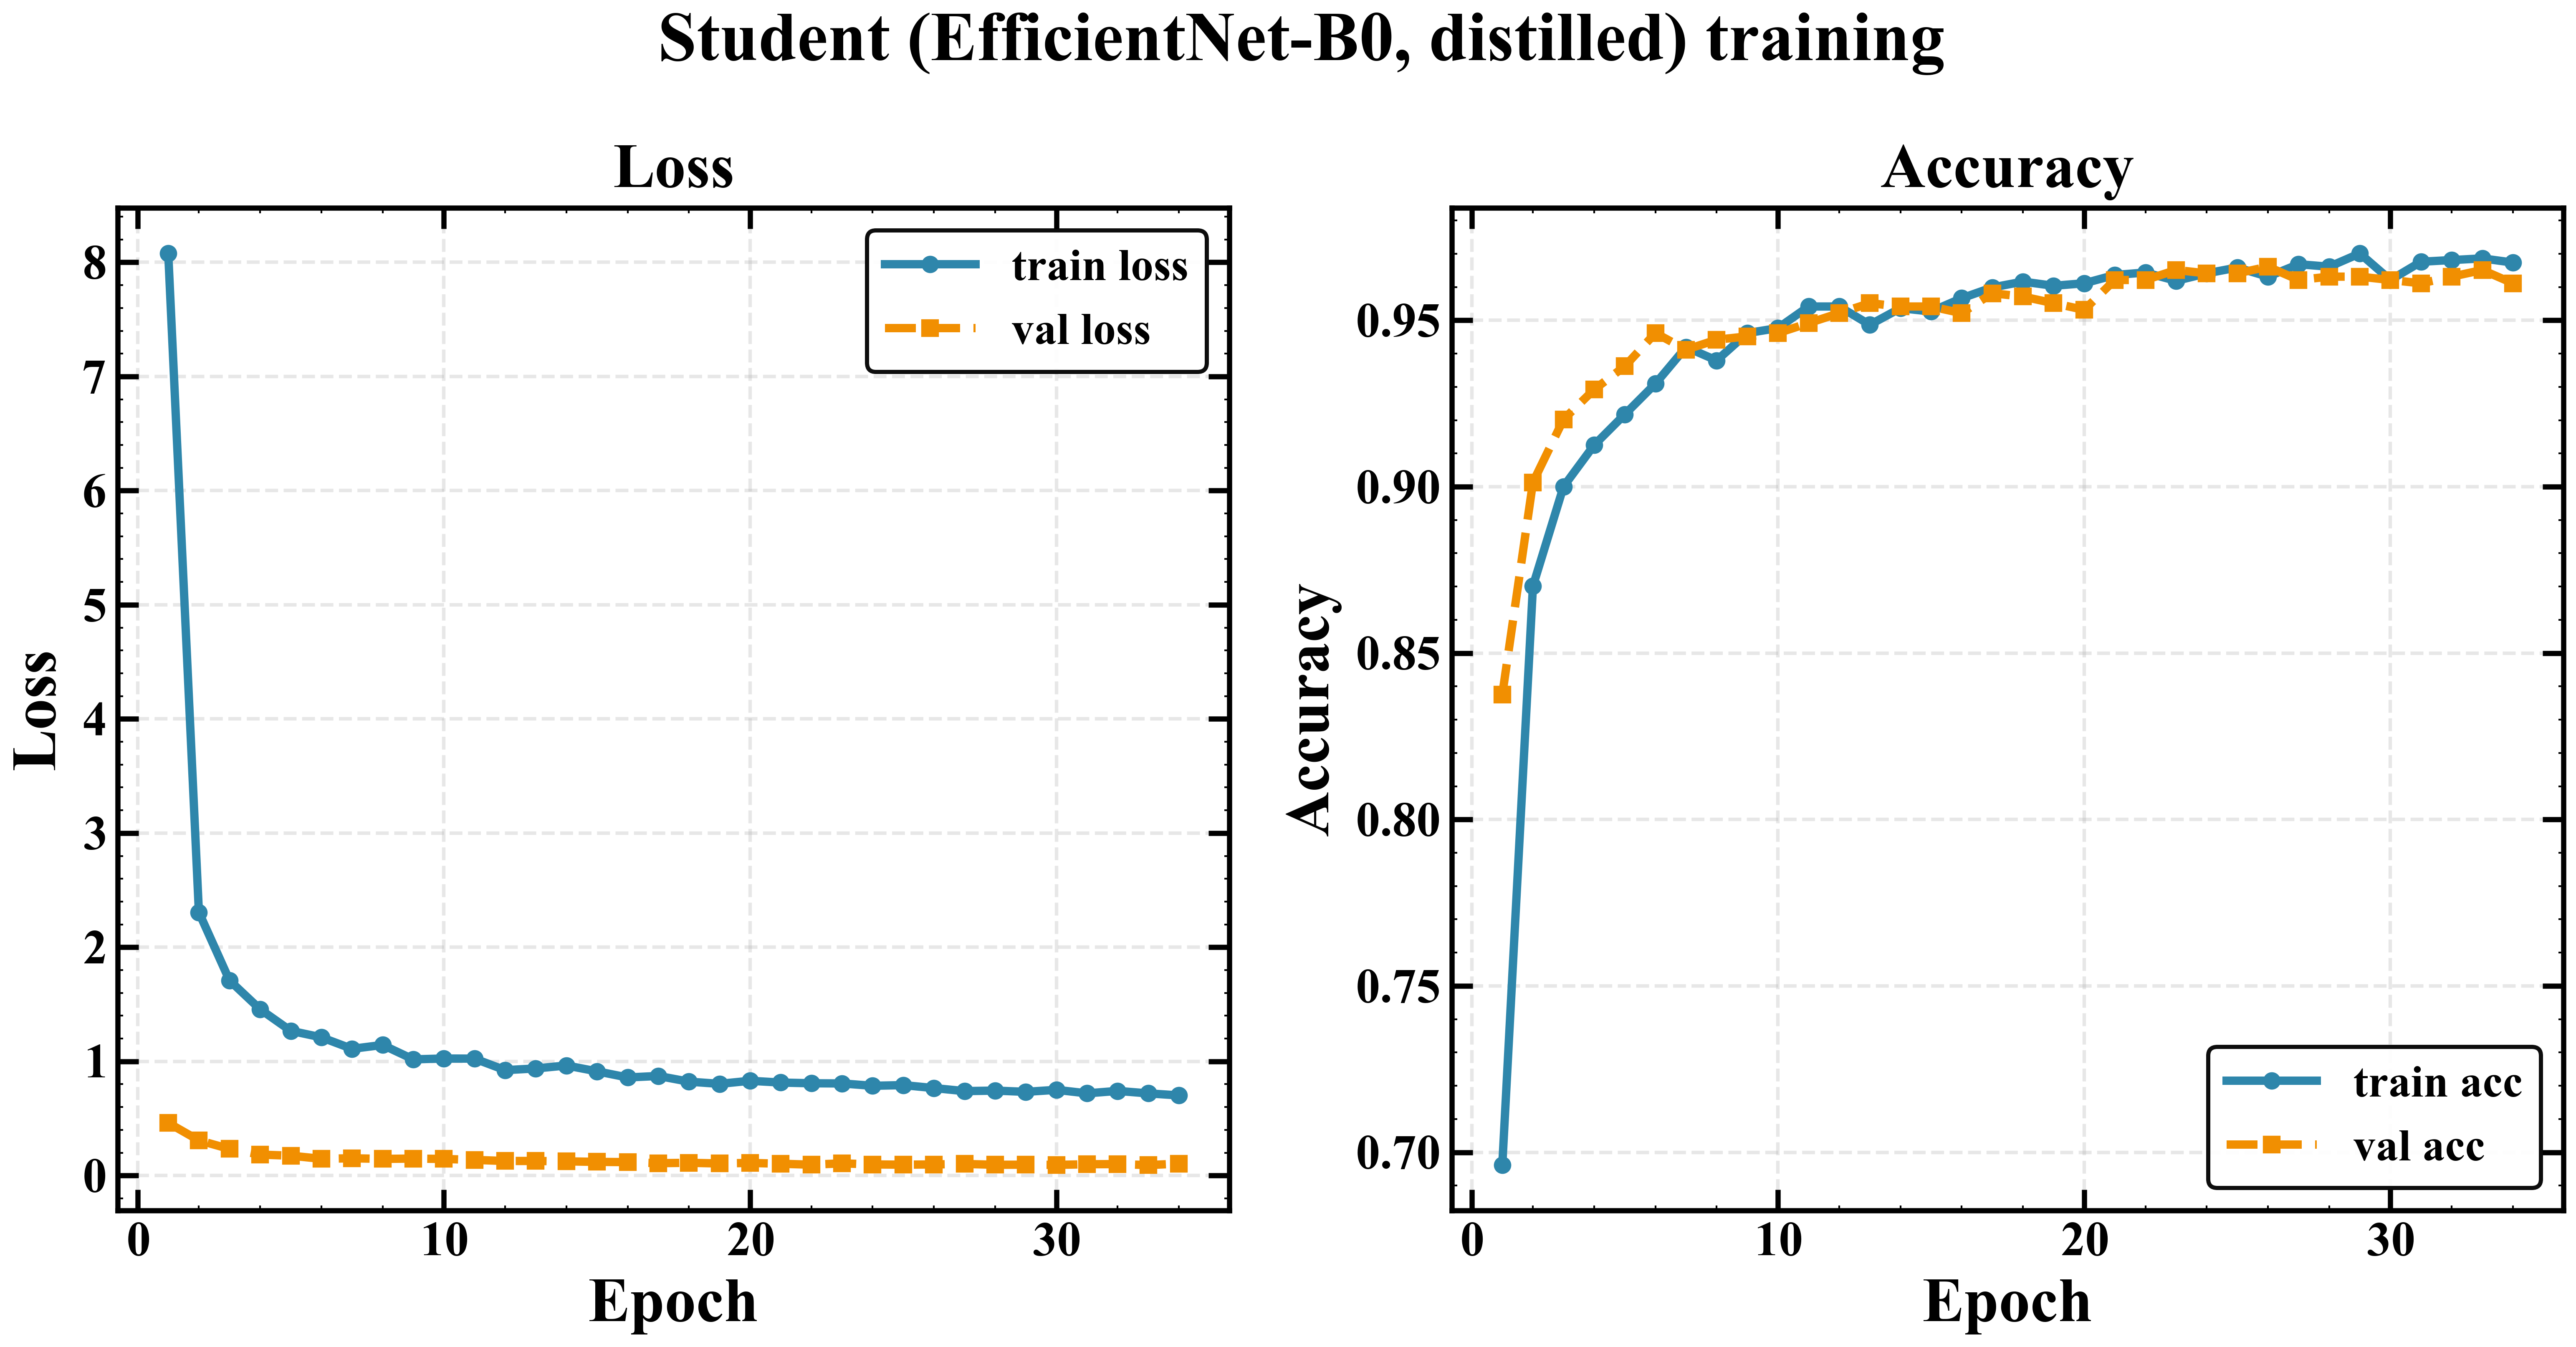
\includegraphics[width=0.49\textwidth]{student_training_curves.png}\hfill
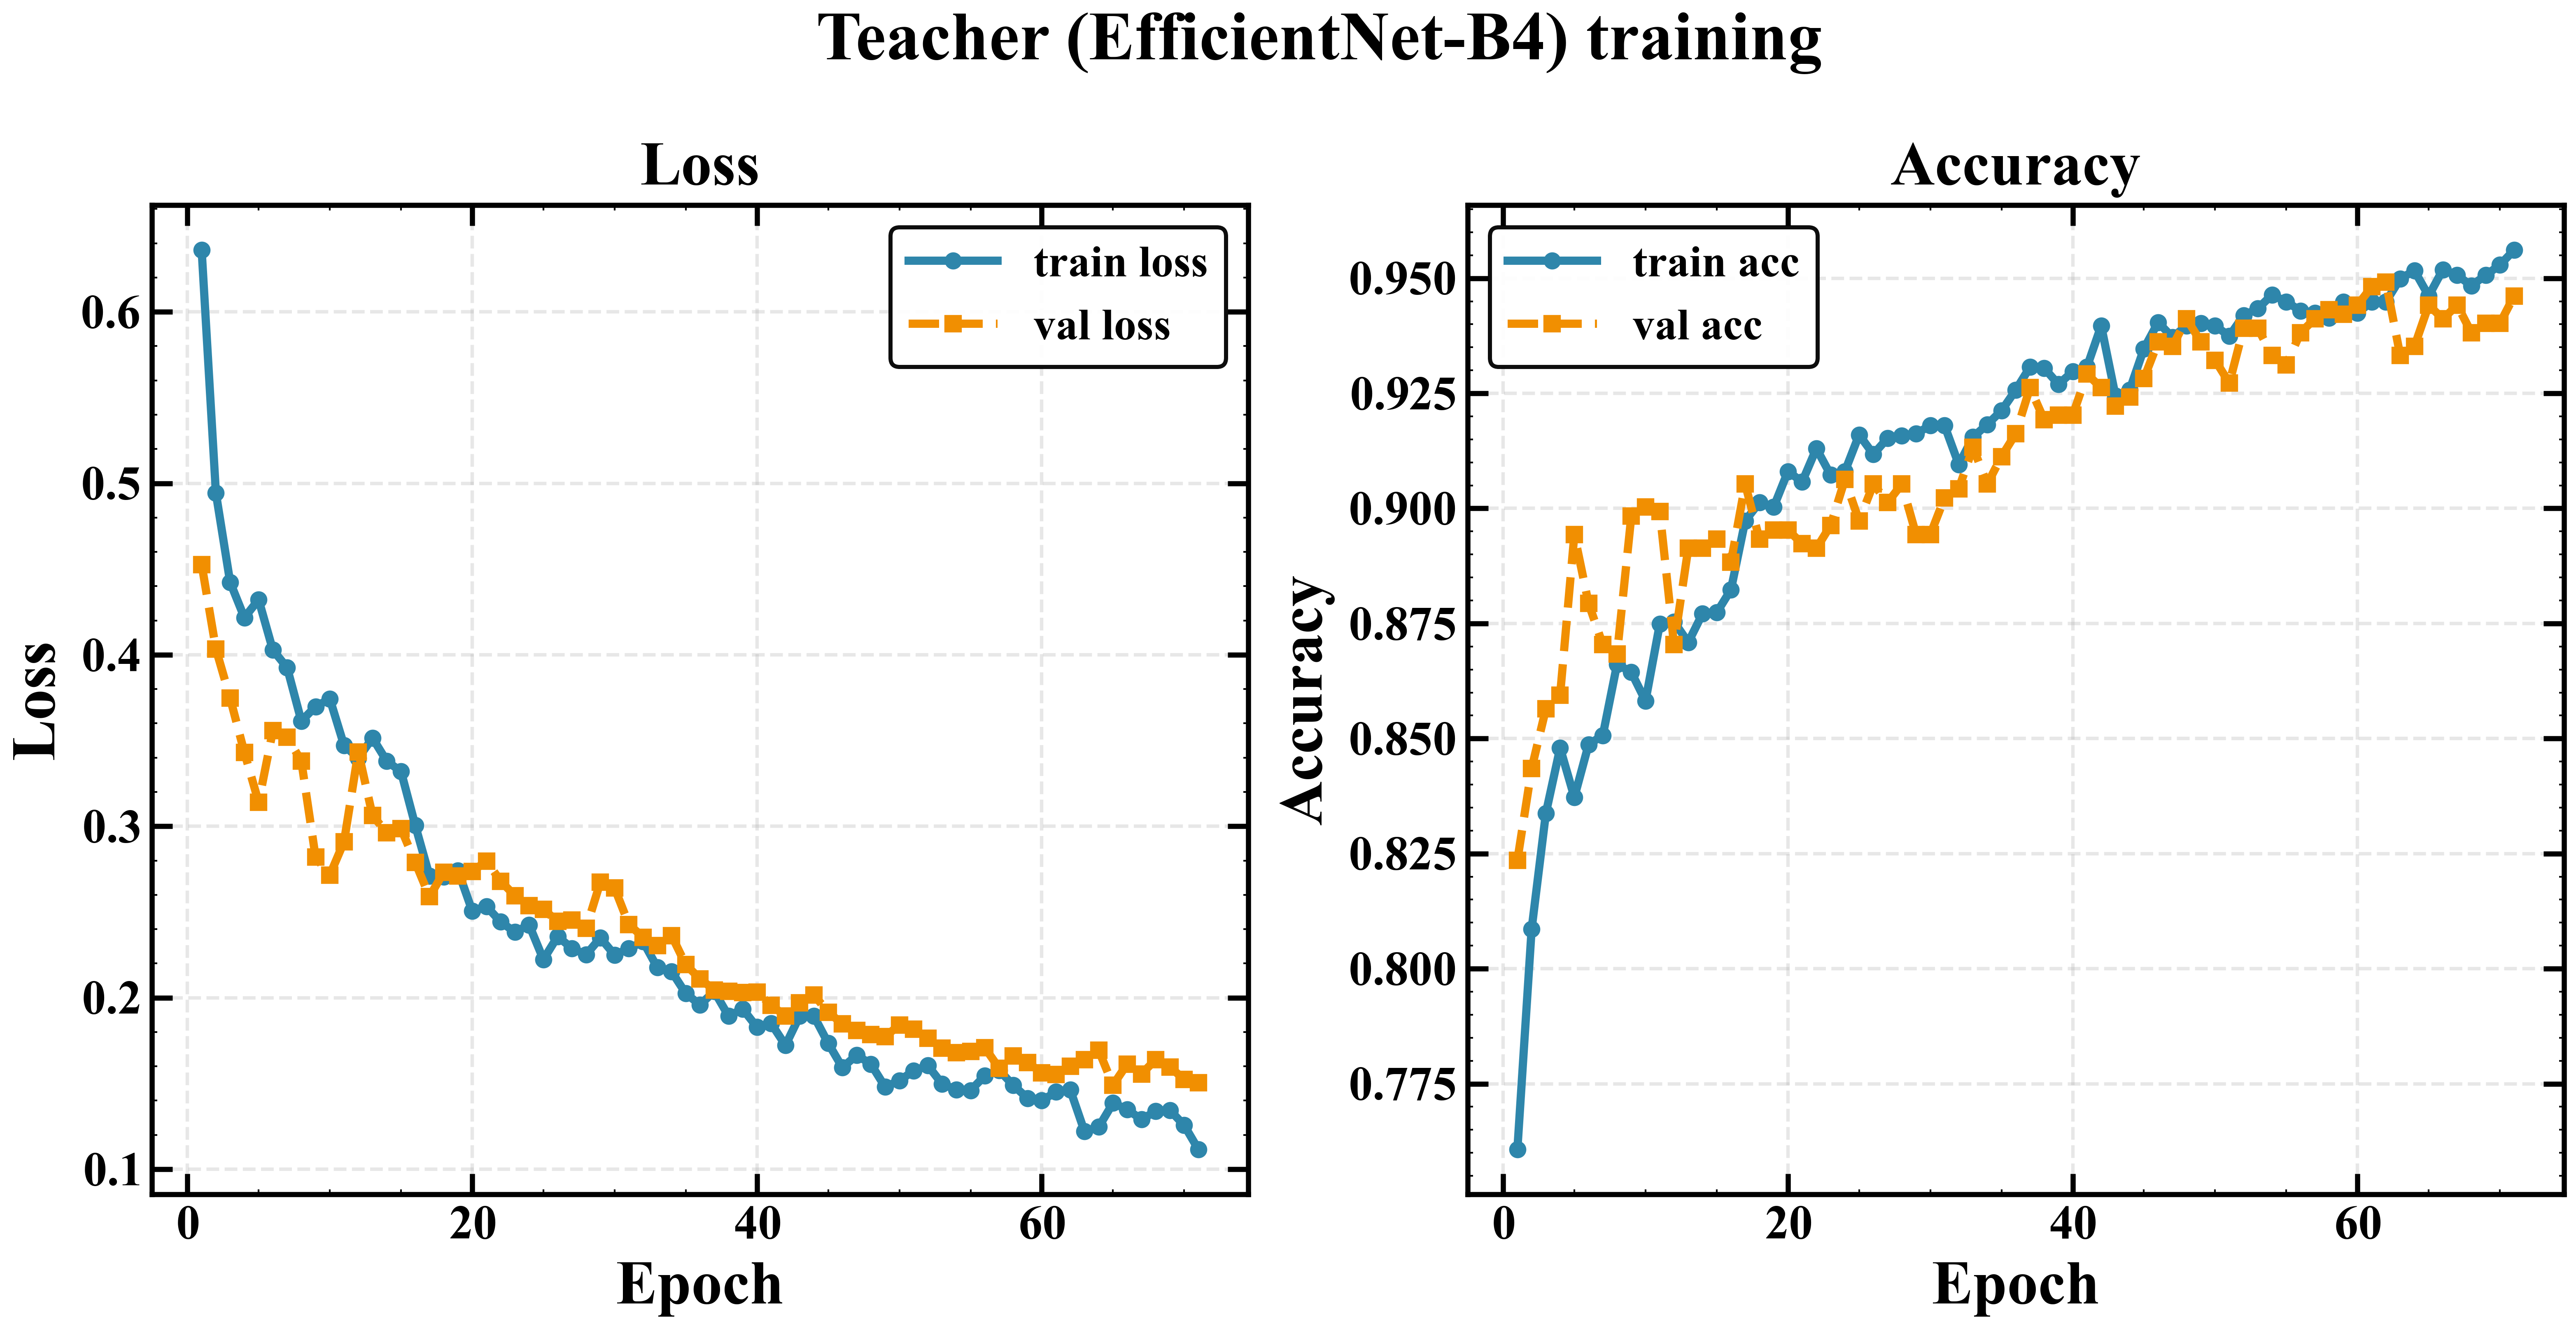
\includegraphics[width=0.49\textwidth]{teacher_training_curves.png}
\caption{Training dynamics. Top: distilled B0 student (34 epochs). Bottom: B4 teacher (two stages, 71 epochs). Validation tracks training in both, indicating no overfitting.}
\label{fig:curves}
\end{figure*}

\begin{table}[t]
\caption{In-distribution five-class metrics on the SIPaKMeD validation split ($n{=}1003$). The
distilled student surpasses its teacher on every metric and remains well calibrated.}
\label{tab:indist}
\centering\small
\begin{tabular}{lcc}
\toprule
Metric & Teacher (B4) & \textbf{Student (B0)} \\
\midrule
Parameters         & 18.5\,M & \textbf{4.67\,M} \\
Accuracy           & 0.943 & \textbf{0.966} \\
Balanced accuracy  & 0.946 & \textbf{0.968} \\
Macro-$F_1$        & 0.945 & \textbf{0.967} \\
Cohen's $\kappa$   & 0.929 & \textbf{0.958} \\
AUROC (OvR macro)  & 0.996 & \textbf{0.998} \\
ECE                & 0.013 & 0.015 \\
\bottomrule
\end{tabular}
\end{table}

\begin{table}[t]
\caption{Per-class precision, recall and $F_1$ for the student on the SIPaKMeD validation split.
Koilocytotic is the weakest class (recall $0.873$), consistent with its morphological overlap.}
\label{tab:perclass}
\centering\small
\begin{tabular}{lcccc}
\toprule
Class & P & R & $F_1$ & $n$ \\
\midrule
Superficial-Intermediate & 0.990 & 1.000 & 0.995 & 191 \\
Parabasal                & 0.989 & 1.000 & 0.994 & 179 \\
Dyskeratotic             & 0.958 & 0.986 & 0.971 & 207 \\
Metaplastic              & 0.933 & 0.981 & 0.957 & 213 \\
Koilocytotic             & 0.969 & 0.873 & 0.919 & 213 \\
\bottomrule
\end{tabular}
\end{table}

\begin{figure}[t]
\centering
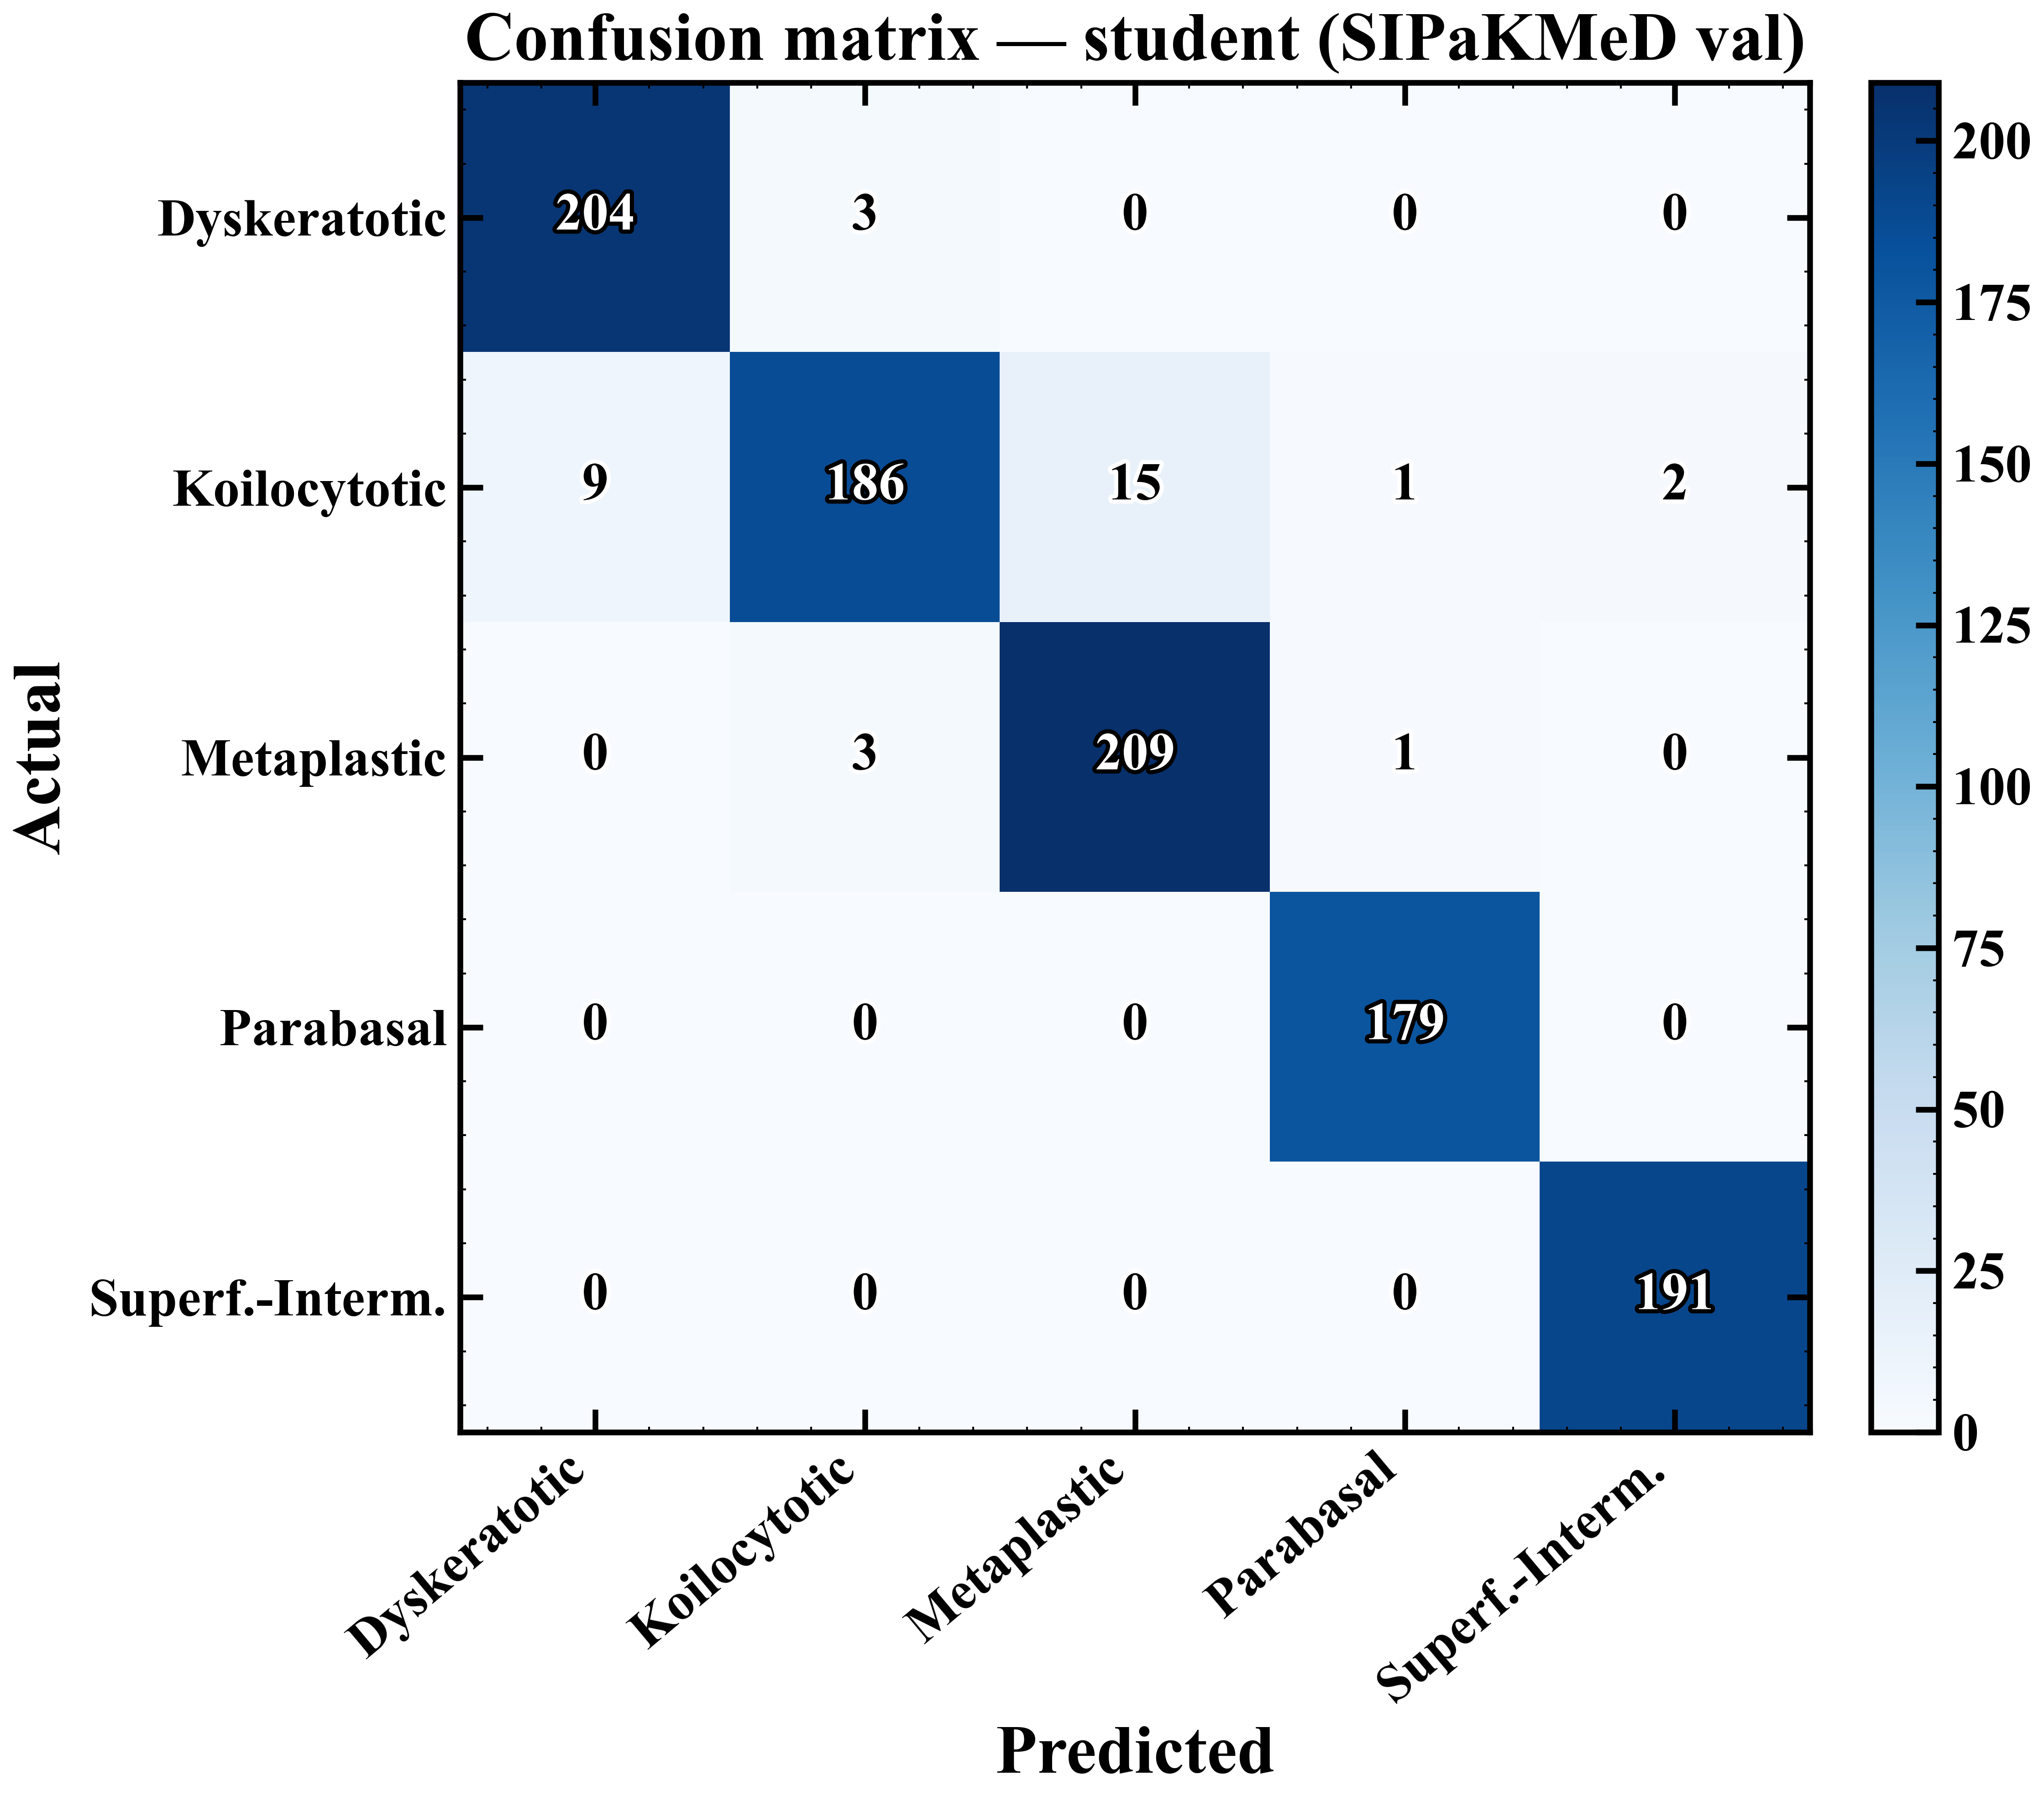
\includegraphics[width=\linewidth]{cm_student.png}
\caption{Five-class confusion matrix (student). Errors concentrate on Koilocytotic.}
\label{fig:cm_student}
\end{figure}

\begin{figure}[t]
\centering
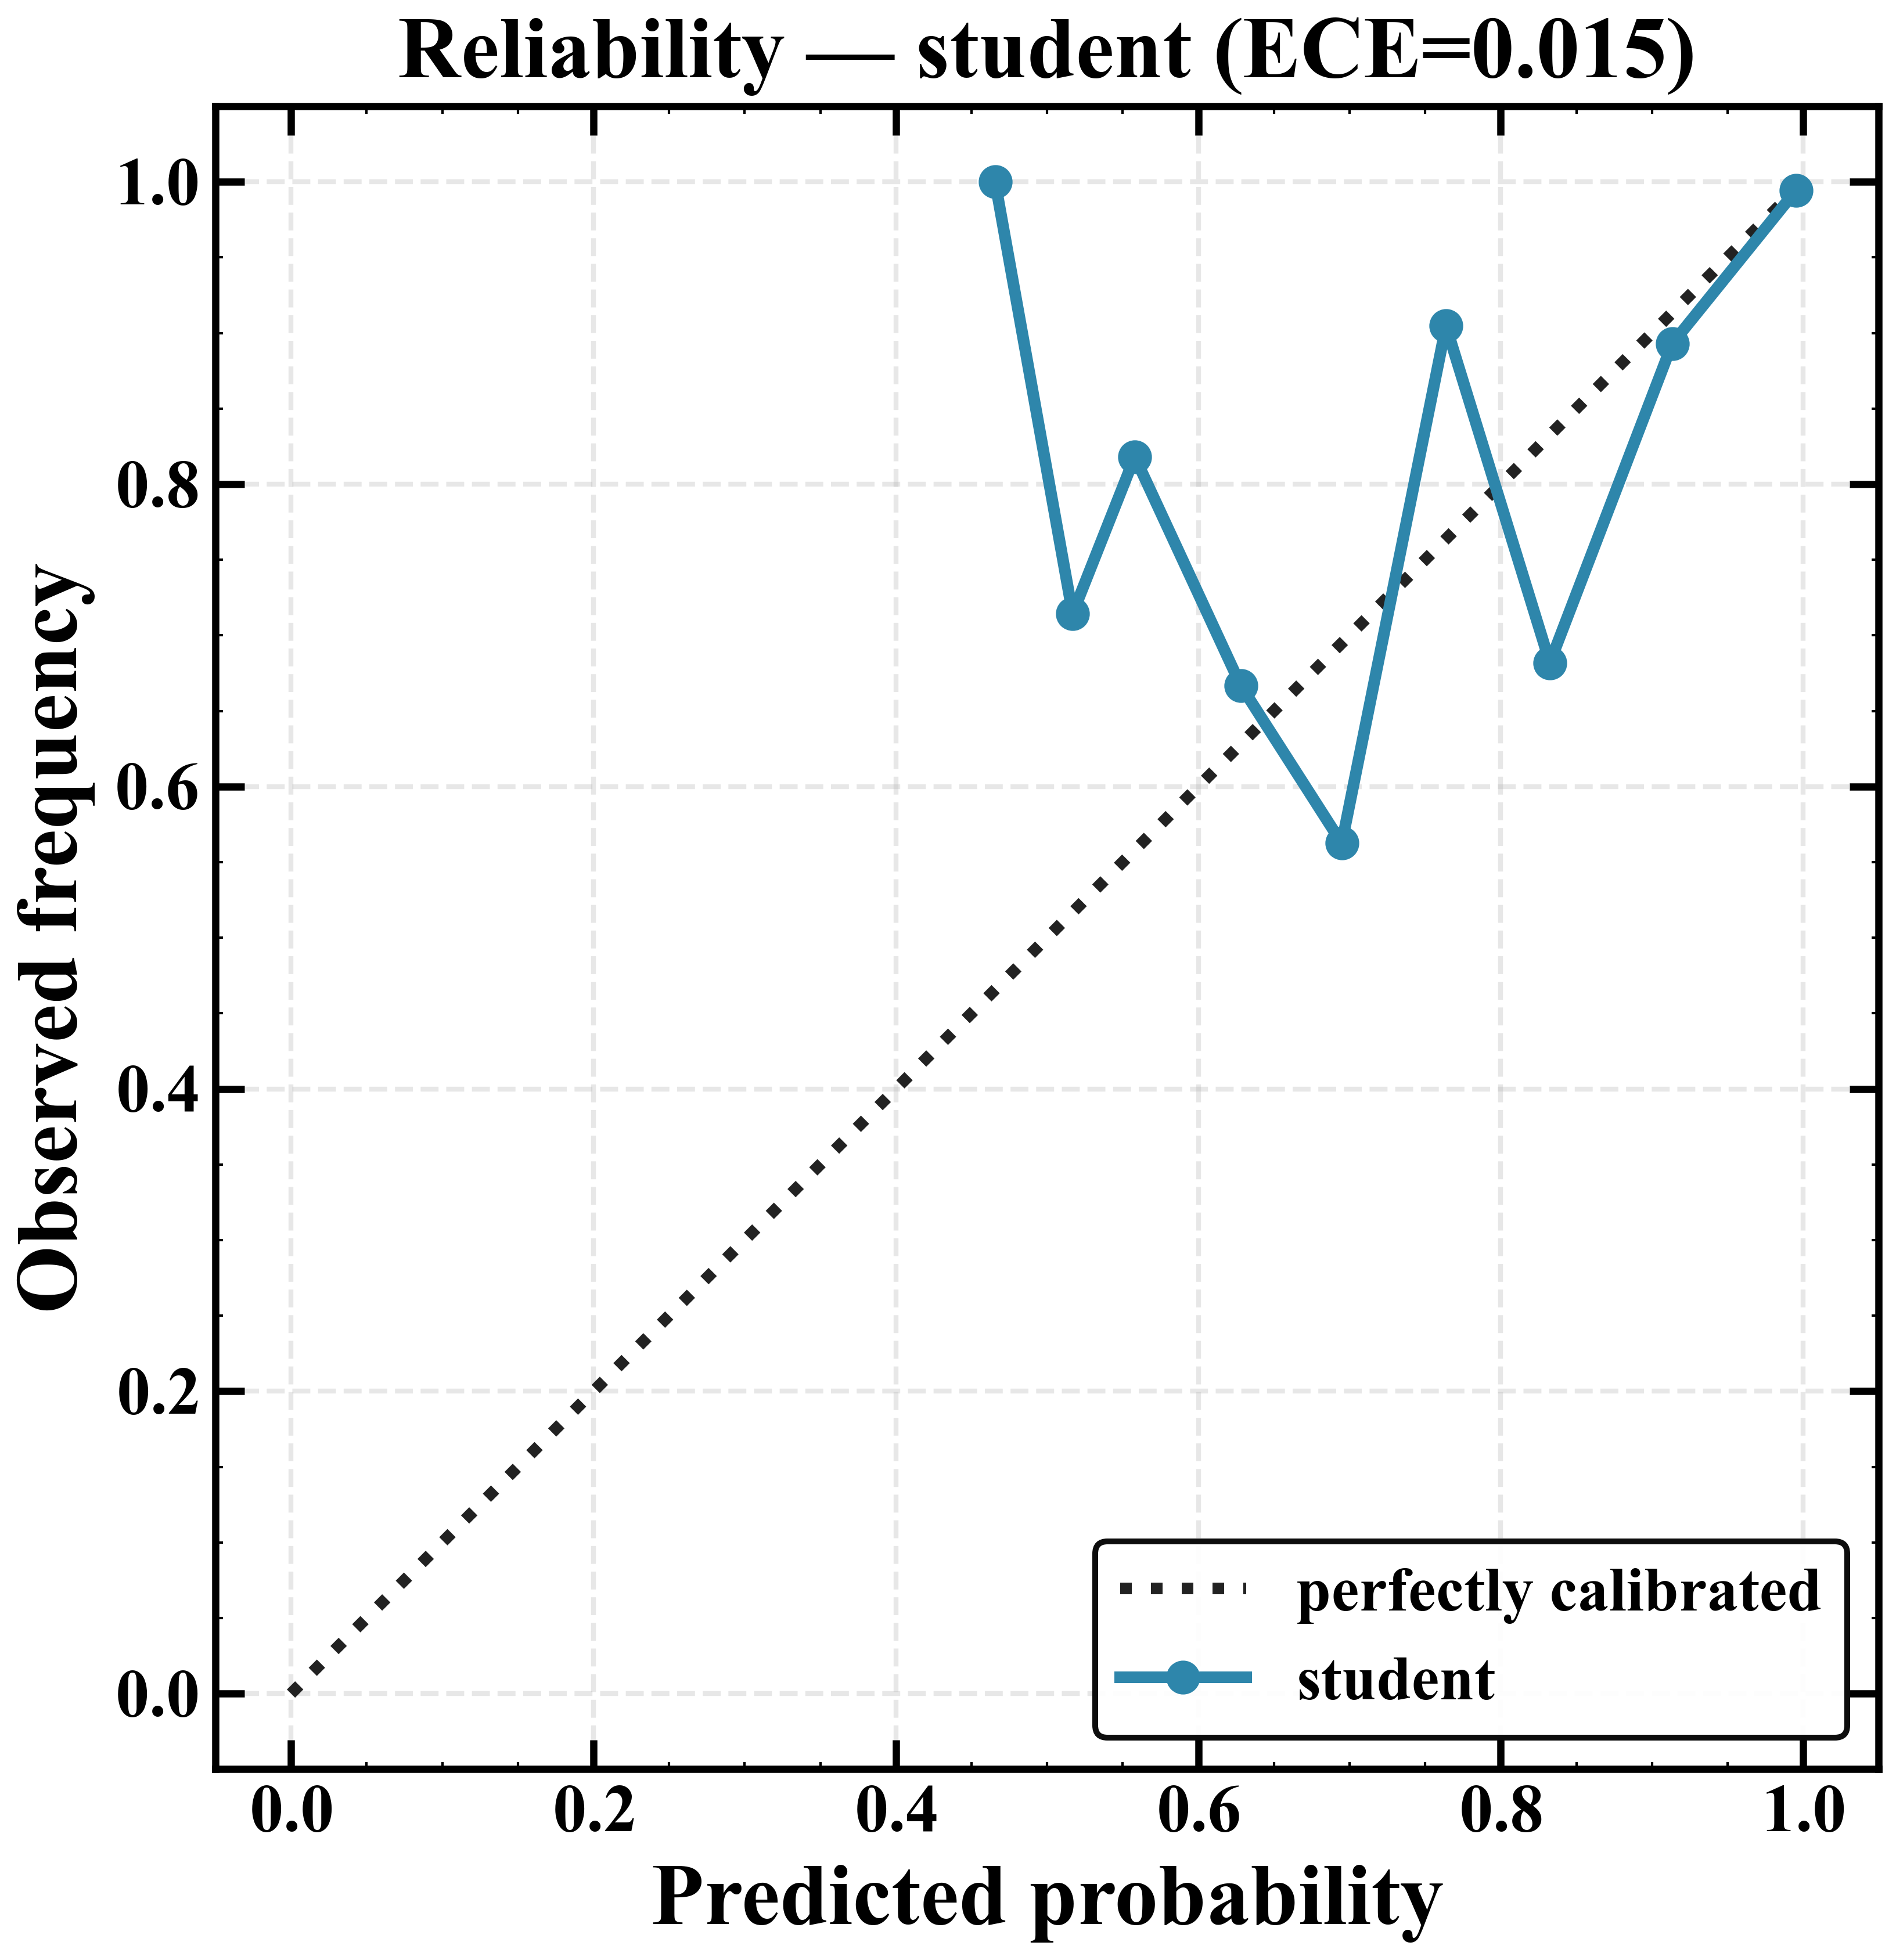
\includegraphics[width=\linewidth]{reliability_student.png}
\caption{Reliability diagram (student, ECE $=0.015$): in-distribution confidence is well calibrated.}
\label{fig:reliability}
\end{figure}

\section{Results: In-distribution}

\subsection{Training dynamics}

Both networks converged stably under the early-stopping regime, and the learning curves in \ref{fig:curves} show no evidence of overfitting: training and validation losses descend in step, and the validation accuracy plateaus rather than degrading after its peak. The teacher required 71 epochs in total, comprising 30 epochs with the backbone frozen followed by 41 epochs of whole-network fine-tuning before early stopping, and reached a final validation accuracy of $0.9442$. The distilled student converged considerably faster, early-stopping after 34 epochs at a final validation accuracy of $0.9661$. The absence of a widening train--validation gap in either curve indicates that the weighted cross-entropy objective for the teacher and the Hinton distillation objective for the student, combined with the augmentation pipeline, were sufficient to regularize models of $18.5$~M and $4.67$~M parameters, respectively, on the $4{,}012$-image training split.

\subsection{Classification performance}

On the held-out SIPaKMeD validation set ($n=1{,}003$), the $4.67$~M-parameter student does not merely approximate its $18.5$~M-parameter teacher; it surpasses it on every metric we report (\ref{tab:indist}). The student attains an accuracy of $0.9661$, balanced accuracy of $0.9680$, macro-F1 of $0.9671$, Cohen's $\kappa$ of $0.9576$, and a one-vs-rest macro AUROC of $0.9981$, against the teacher's $0.9432$, $0.9458$, $0.9449$, $0.9289$, and $0.9955$. That a model with roughly one-quarter of the teacher's parameters improves on it across accuracy, agreement, and ranking metrics is consistent with the regularizing effect of knowledge distillation, whereby the soft teacher targets convey inter-class similarity structure that a hard one-hot objective discards, answering RQ1 affirmatively: the distilled student matches and indeed exceeds the teacher at a fraction of the parameter budget.

The per-class breakdown (\ref{tab:perclass}) and the confusion matrix in \ref{fig:cm_student} locate the student's residual error. Performance is near-saturated on the two morphologically distinctive normal classes, with F1 scores of $0.995$ for Superficial-Intermediate and $0.994$ for Parabasal, and remains strong for Dyskeratotic ($0.971$) and Metaplastic ($0.957$). The clear weak point is the Koilocytotic class, whose F1 of $0.919$ is driven by a recall of only $0.873$: roughly one in eight koilocytotic cells is misassigned, predominantly to its morphological neighbours. This is cytologically unsurprising, as koilocytotic change---perinuclear haloing and nuclear atypia of intermediate severity---occupies a continuum between the metaplastic and dyskeratotic appearances rather than a sharply separable region of feature space, so the confusions concentrate exactly where human graders also disagree. Notably, Koilocytotic is also the teacher's weakest class (F1 $0.877$), and the student's improvement here ($+0.042$ F1) accounts for much of its overall margin over the teacher.

\subsection{Calibration}

Strong discrimination is matched by faithful confidence estimates. The student's $15$-bin Expected Calibration Error is $0.0152$, and the reliability diagram in \ref{fig:reliability} tracks the identity line closely across the confidence range, indicating that predicted probabilities can be read as approximately trustworthy likelihoods of correctness. The teacher is marginally better calibrated still, with an ECE of $0.0131$, so the small calibration cost of distillation is more than offset by the student's gains in discrimination. We emphasize that this in-distribution calibration is established on SIPaKMeD itself; whether it transfers to independent datasets is precisely the question taken up in the cross-dataset analysis, and the answer there is markedly less favourable.


\begin{figure*}[t]
\centering
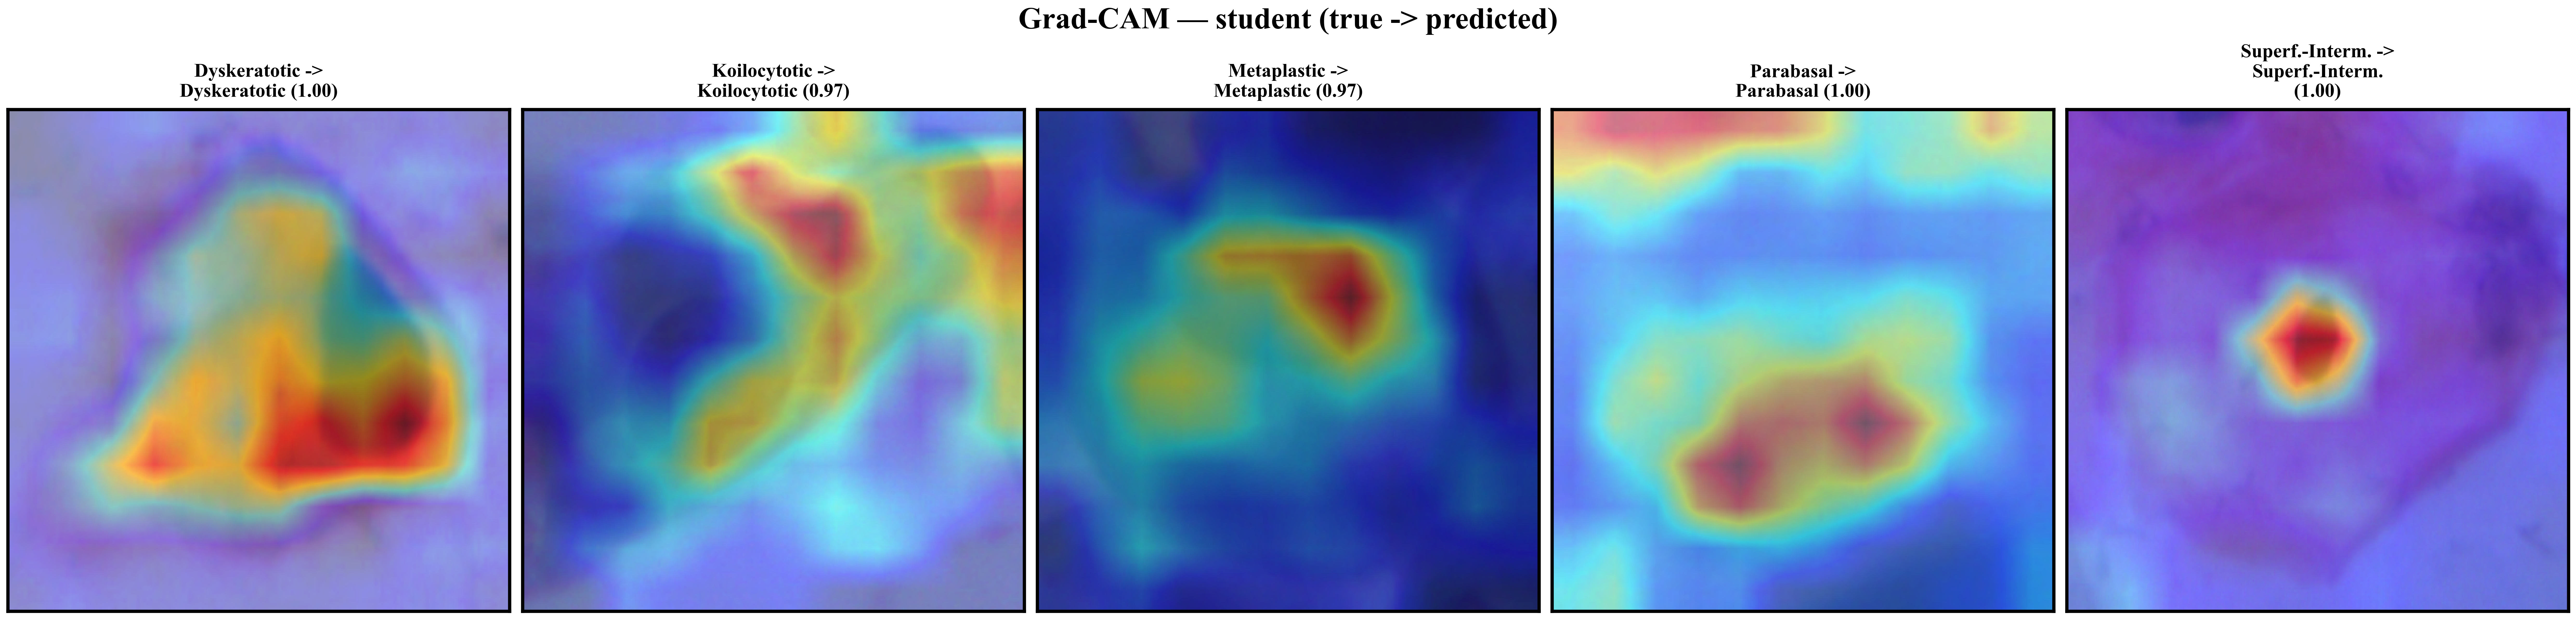
\includegraphics[width=\textwidth]{gradcam_student.png}
\caption{Grad-CAM for the student, one representative cell per class (true $\rightarrow$ predicted, confidence). Heatmaps localize to nuclear/cellular regions.}
\label{fig:gradcam}
\end{figure*}

\begin{table*}[t]
\caption{Cross-dataset binary (Normal/Abnormal) results for the student (internal SIPaKMeD accuracy
$0.966$). $\Delta P$ is the separation between mean $P(\mathrm{abnormal})$ on true-abnormal vs.\
true-normal cells (positive $=$ correct ordering); ``Maj.'' is the majority-class baseline. At
$\tau{=}0.5$ accuracy falls \emph{below} the majority baseline for Herlev and HiCervix despite
AUROC$>0.5$.}
\label{tab:cross}
\centering\small
\begin{tabular}{lccccccc}
\toprule
Dataset & $n$ & Acc & Bal.\ acc & Sens & Spec & AUROC & $\Delta P$ \\
\midrule
Herlev   & 917  & 0.639 & 0.651 & 0.625 & 0.678 & \textbf{0.728} & $+0.284$ \\
HiCervix & 4823 & 0.605 & 0.562 & 0.386 & 0.738 & 0.594 & $+0.112$ \\
APACC    & 1125 & 0.532 & 0.535 & 0.654 & 0.417 & 0.525 & $+0.045$ \\
\midrule
\multicolumn{8}{l}{\footnotesize Internal SIPaKMeD: Acc $0.966$ \quad|\quad Maj.\ baselines: Herlev $0.74$, HiCervix $0.62$, APACC $0.51$.}\\
\bottomrule
\end{tabular}
\end{table*}

\begin{figure*}[t]
\centering
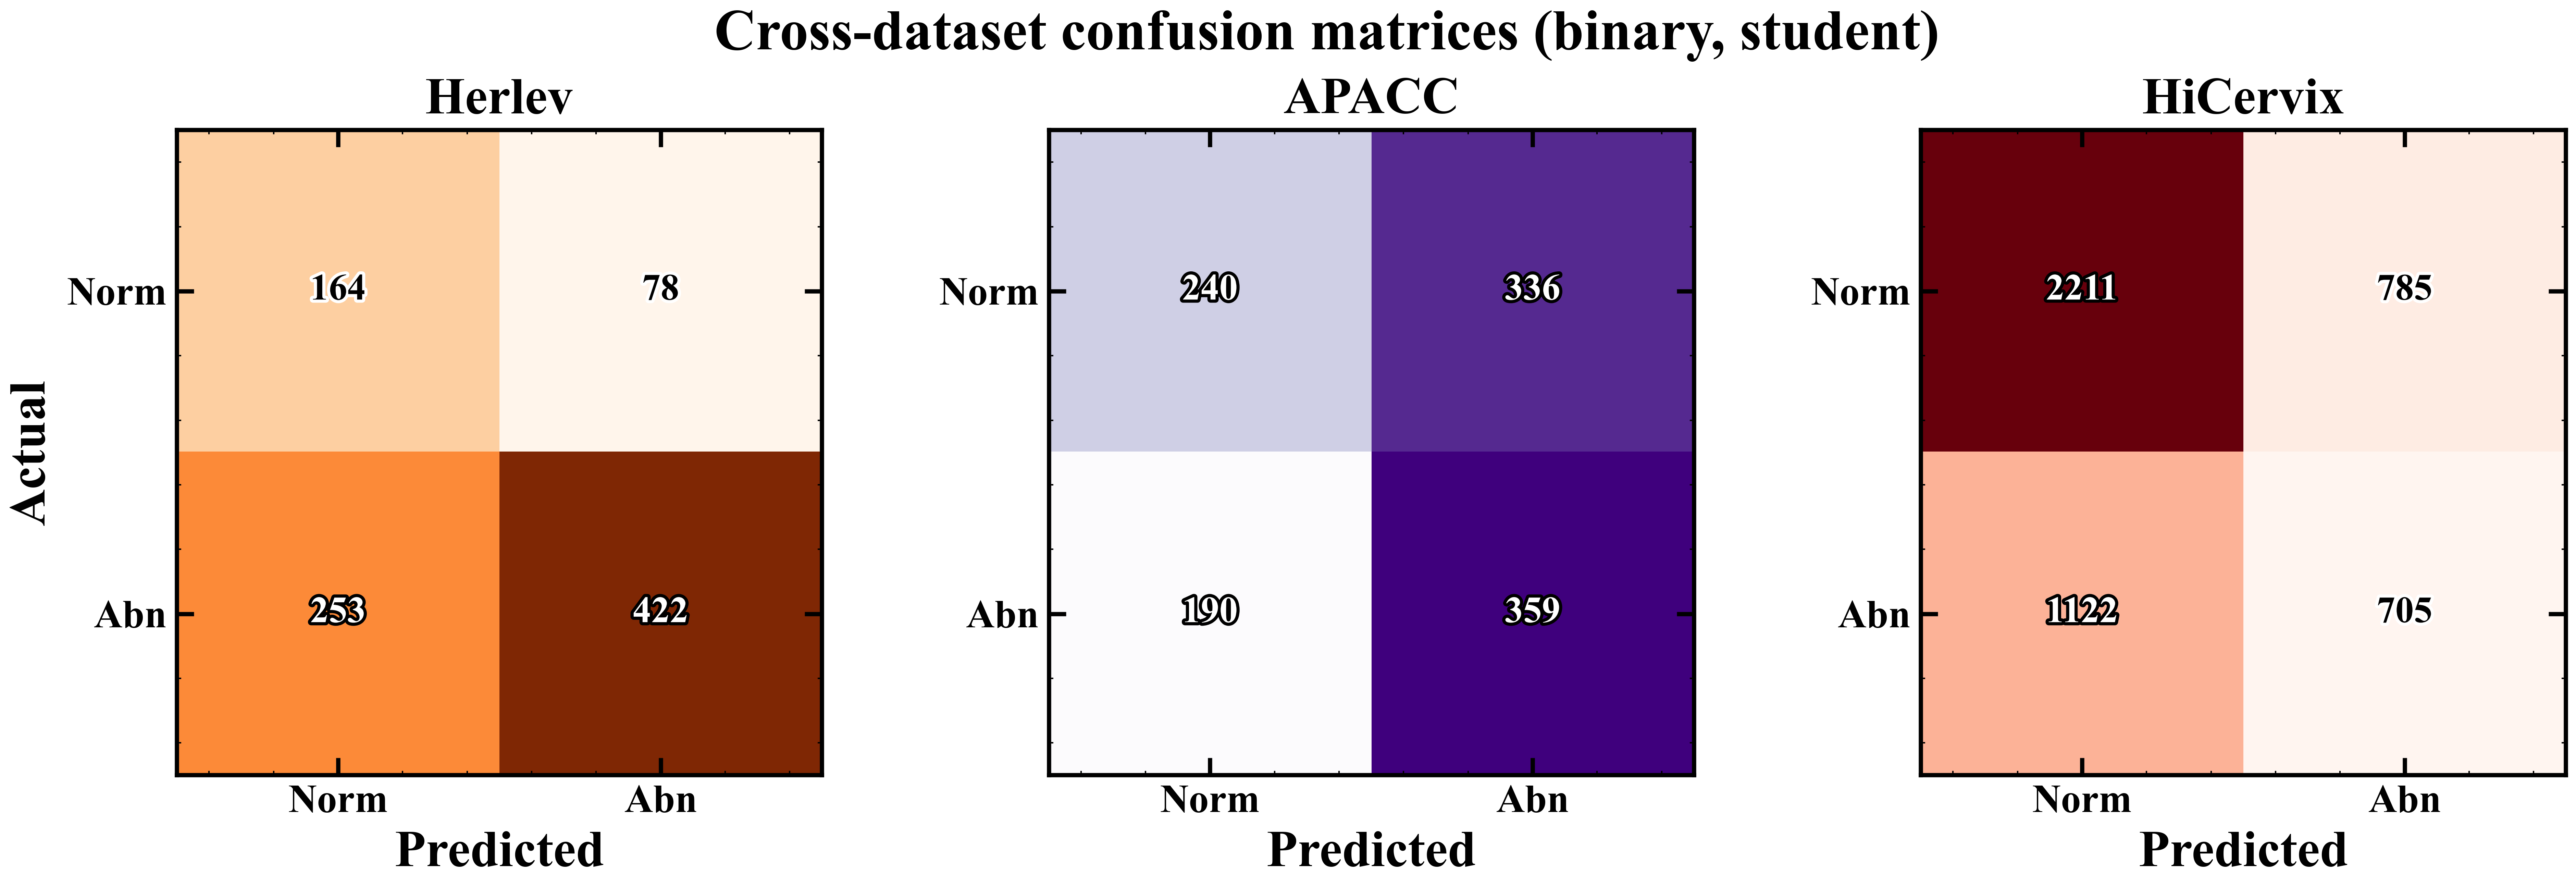
\includegraphics[width=\textwidth]{cm_cross_combined.png}
\caption{Cross-dataset binary confusion matrices: the model over-predicts \emph{abnormal} on APACC (low specificity) and \emph{normal} on HiCervix (low sensitivity).}
\label{fig:cmcross}
\end{figure*}

\begin{figure*}[t]
\centering
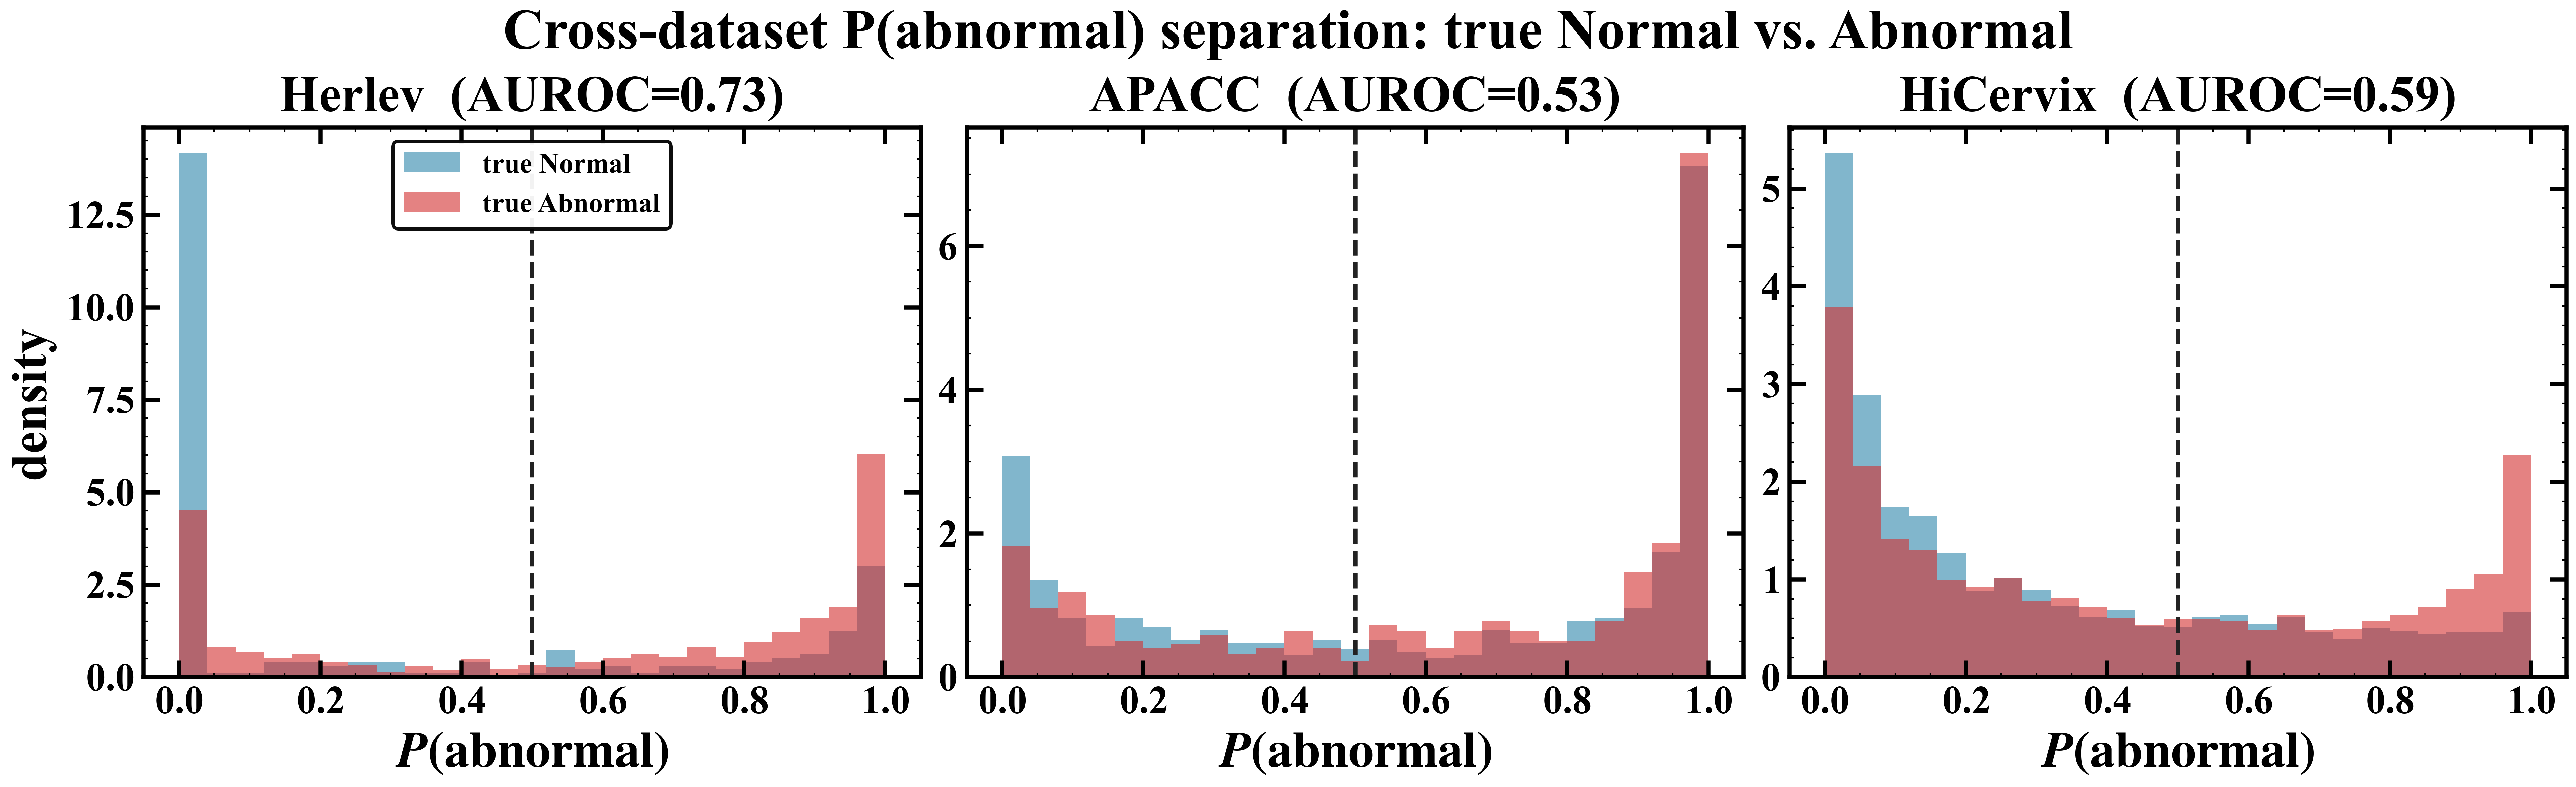
\includegraphics[width=\textwidth]{cross_separation.png}
\caption{Distribution of $P(\mathrm{abnormal})$ for true-normal (blue) vs.\ true-abnormal (red) cells. Separation is clear on Herlev, weak on HiCervix and absent on APACC; the dashed line is $\tau{=}0.5$.}
\label{fig:sep}
\end{figure*}

\section{Results: Explainability and Cross-dataset Generalization}

\subsection{Grad-CAM}

To interrogate whether the student's in-distribution accuracy rests on cytologically meaningful evidence rather than incidental background cues, we visualized class-discriminative attention with Grad-CAM \citep{selvaraju2017gradcam} applied to the final convolutional block of the EfficientNet-B0 student. Figure~\ref{fig:gradcam} presents one representative cell from each of the five SIPaKMeD classes. All five exemplars were classified correctly, and at high confidence (predicted-class probability between $0.97$ and $1.00$), so the visualizations report attention for decisions the model got right rather than rationalizations of errors. Across every panel the salient regions concentrate on the nucleus and the surrounding cytoplasmic body, the same structures a cytotechnologist inspects when assessing nuclear enlargement, hyperchromasia, perinuclear haloing, and keratinization. The heatmaps do not localize to slide background, staining gradients, or crop borders, which would have signalled shortcut learning of the kind that frequently inflates apparent performance on medical-image benchmarks \citep{geirhos2020shortcut}. We therefore read these attributions as evidence that the in-distribution decision surface is anchored to plausible cellular morphology. This interpretation carries an important caveat: Grad-CAM is a saliency-attribution method that reports \emph{where} gradient-weighted activations are strongest, not \emph{why} a clinical category was chosen. Spatial overlap with the nucleus is consistent with sound reasoning but does not constitute a faithfulness guarantee, and it says nothing about whether the learned features survive a change of imaging domain---the question we turn to next.

\subsection{Cross-dataset performance}

Against the $0.966$ accuracy achieved within SIPaKMeD, performance on three independent external Pap datasets collapses toward chance. Table~\ref{tab:cross} reports the binary Normal-versus-Abnormal results and Figure~\ref{fig:cmcross} the corresponding confusion matrices. On Herlev \citep{jantzen2005herlev} ($n=917$) the model reaches accuracy $0.639$, balanced accuracy $0.651$, sensitivity $0.625$, specificity $0.678$, and AUROC $0.728$. On HiCervix \citep{cai2024hicervix} ($n=4823$) accuracy falls to $0.605$ with balanced accuracy $0.562$, a markedly depressed sensitivity of $0.386$, specificity $0.738$, and AUROC $0.594$. On APACC ($n=1125$) the model is effectively at chance: accuracy $0.532$, balanced accuracy $0.535$, sensitivity $0.654$, specificity $0.417$, and AUROC $0.525$. The internal-to-external degradation is therefore on the order of $33$ accuracy points in the most favourable case and larger elsewhere, and the discriminative ranking signal weakens monotonically from Herlev through HiCervix to APACC. This is the answer to RQ2 and confirms H2: strong, well-calibrated in-distribution accuracy does not, on its own, translate into cross-dataset generalization.

\subsection{Why cross-dataset evaluation fails}

We disentangle four contributing factors, and crucially distinguish a genuine model and domain failure from a mere artefact of our label crosswalk. \emph{First, the collapse is not a labelling artefact.} The class-conditional separation of the predicted abnormality score, $\Delta = \overline{P(\text{abnormal})}_{\text{abnormal}} - \overline{P(\text{abnormal})}_{\text{normal}}$, is positive on every dataset---$+0.284$ on Herlev, $+0.112$ on HiCervix, and $+0.045$ on APACC (Figure~\ref{fig:sep})---and all three AUROC values exceed $0.5$. Had our many-to-one mapping been inverted or ill-defined, the model would have ranked abnormal cells \emph{below} normal ones, yielding $\Delta<0$ and AUROC$<0.5$; instead the ordering is preserved, weakly but consistently, in the direction the mapping intends. Combined with an explicit audit of each mapper, this rules out relabelling as the cause (RQ3, H3).

\emph{Second, the dominant failure is operating-point miscalibration.} The in-distribution calibration (ECE $0.0152$) does not transfer: the baseline level of $P(\text{abnormal})$ shifts per domain, sitting high (around $0.6$) on APACC so the fixed threshold $\tau=0.5$ over-calls abnormality, and low (around $0.35$) on HiCervix so it under-calls it. A single global threshold consequently discards the ranking information the AUROC shows is present. The symptom is diagnostic: at $\tau=0.5$ accuracy falls \emph{below} the majority-class baseline for Herlev ($0.639$ vs.\ $0.74$) and HiCervix ($0.605$ vs.\ $0.62$), even though AUROC $>0.5$. Re-tuning $\tau$ on the test labels as an oracle recovers $0.75$ on Herlev (at $\tau=0.05$), $0.65$ on HiCervix (at $\tau=0.85$), and $0.53$ on APACC (at $\tau=0.40$)---confirming that much of the deficit is threshold placement rather than absent signal, and answering RQ4 (H4): calibration holds in-distribution but does not transfer.

\emph{Third, the residual signal degrades with slide-preparation distance from SIPaKMeD's conventional smear.} Threshold-free AUROC tracks this gradient cleanly: Herlev (conventional Pap) $0.728$ $>$ HiCervix (liquid-based cytology) $0.594$ $>$ APACC (auto-segmented noisy crops) $0.525\approx$ chance, indicating that preparation and segmentation domain shift, not labels, erode the discriminative features. \emph{Fourth, the internal $0.966$ is itself optimistic.} It derives from a random per-cell split that can place cells from the same cluster field-of-view on both sides of the train/validation boundary; a leakage-safe, cluster-grouped split would lower the internal figure, so the true internal-to-external gap is larger still than the headline numbers suggest. Together these factors recast the cross-dataset collapse as a problem of domain shift and operating-point transfer---addressable by stain and domain normalization \citep{macenko2009stain}, per-domain calibration \citep{guo2017calibration}, leakage-aware evaluation, and threshold-free reporting---rather than as a flaw in the label alignment.

\section{Discussion}

The central finding of this audit is a stark dissociation between in-distribution competence and cross-dataset generalization. Within SIPaKMeD, the distilled EfficientNet-B0 student is an accurate, well-calibrated, and visually faithful five-class classifier: it reaches an accuracy of $0.966$, a macro-F1 of $0.967$, a one-vs-rest AUROC of $0.998$, and an Expected Calibration Error of only $0.015$, with Grad-CAM attributions consistently localized to nuclear and cytoplasmic structure rather than background artefacts. Yet when this same model is confronted with three independent Papanicolaou datasets under a deterministic binary Normal/Abnormal alignment, performance collapses toward, and in places below, majority-class baselines: binary accuracy falls to $0.639$ on Herlev, $0.605$ on HiCervix, and $0.532$ on APACC, the latter essentially indistinguishable from chance (AUROC $0.525$). The roughly thirty-three-point internal-to-external gap is the empirical heart of this paper, and it directly answers RQ2 in the negative: strong within-dataset accuracy does not translate into deployable cross-dataset performance.

It is important to read the student-exceeds-teacher result in the correct light. The B0 student surpasses its B4 teacher on every in-distribution metric---accuracy ($0.966$ versus $0.943$), balanced accuracy, macro-F1, kappa, AUROC, and calibration---at roughly a quarter of the parameters ($4.67$\,M versus $18.5$\,M). Consistent with the regularizing view of knowledge distillation \citep{hinton2015distilling}, the soft-target signal appears to smooth the student's decision boundaries and improve generalization \emph{within the training distribution}. This is a genuine efficiency win and confirms H1. However, the same audit shows that this advantage is confined to the source domain: a better in-distribution model is not a more transportable one. Distillation optimizes agreement with a teacher trained on SIPaKMeD, and any domain-specific shortcuts \citep{geirhos2020shortcut} the teacher encodes are inherited, not corrected, by the student.

The diagnosis isolates the failure mechanism and, crucially, exonerates the label crosswalk. Because the class-conditional separation of $P(\text{abnormal})$ is positive in all three datasets ($+0.284$ Herlev, $+0.112$ HiCervix, $+0.045$ APACC) and every AUROC exceeds $0.5$, the mappings cannot be inverted or mis-specified---a flipped alignment would drive AUROC below $0.5$. The model therefore retains \emph{some} valid ranking signal everywhere; what it loses is the operating point. The exemplary in-distribution calibration does not transfer: the baseline of $P(\text{abnormal})$ drifts per domain, sitting high on APACC (the model over-calls abnormal) and low on HiCervix (it under-calls), so a fixed threshold $\tau=0.5$ throws away the surviving ranking and pushes accuracy beneath the majority baseline. The oracle best-threshold analysis quantifies this calibration gap precisely---Herlev recovers to $0.75$ at $\tau=0.05$, HiCervix to $0.65$ at $\tau=0.85$---and confirms that miscalibration, not loss of discriminative information, is the dominant culprit. This resolves RQ3 in favour of H3: the collapse is genuine domain shift compounded by operating-point miscalibration, not a relabelling artefact. The ordering of degradation by slide-preparation distance---conventional Herlev $>$ liquid-based HiCervix $>$ auto-segmented APACC---further implicates stain and preparation domain shift as the underlying axis.

For screening deployment the implications are sobering and concrete. A model validated only within its source dataset, however impressive its headline numbers, can silently degrade to chance on the next site's slides, and a fixed decision threshold is actively harmful because calibration is the first thing to break. The remedies follow directly from the diagnosis. First, evaluation must be leakage-safe: same-field-of-view cells should be grouped so that no cluster straddles the train/validation boundary, since the random per-cell split renders even the $0.966$ internal figure optimistic and widens the true gap. Second, stain and domain normalization at input \citep{macenko2009stain} should be used to shrink the preparation distance that drives the degradation ordering. Third, because the ranking signal survives but the operating point does not, per-domain recalibration of the threshold or of the probabilities themselves \citep{guo2017calibration} is essential before any fixed cut-off is trusted on a new site. Finally, reporting practice should favour threshold-free AUROC alongside the excluded fraction, so that discriminative ability and label-space honesty are both visible rather than masked by a single, non-transportable accuracy.

\subsection{Limitations}

Several limitations bound these conclusions. First, the model is trained on a single source dataset (SIPaKMeD); the failure modes we characterize are therefore relative to one conventional-smear domain, and we cannot disentangle how much of the collapse a multi-source training corpus would absorb. Second, the in-distribution metrics rest on a random per-cell $80/20$ split that leaks same-field-of-view cells across train and validation; the reported $0.966$ is consequently optimistic, the genuine internal-to-external gap is larger than the headline thirty-three points, and we quantify the direction but not the exact magnitude of this leakage. Third, the cross-dataset evaluation collapses rich dysplasia and Bethesda gradings into a binary Normal/Abnormal axis---the only label level that is deterministically and many-to-one mappable across schemes---which necessarily discards high-grade detail: severity gradients, glandular lesions (AGC, Herlev columnar), and microbial categories are either excluded or flattened, so the binary numbers cannot speak to high-grade lesion detection specifically. Fourth, Grad-CAM evidence is attribution rather than proof of clinical reasoning, and the qualitative panel covers one representative cell per class. Finally, this is an algorithmic audit on retrospective public datasets with no prospective clinical validation, no reader study, and no assessment on prospectively collected slides; the remedies we propose are evidence-led hypotheses for closing the gap, not validated deployment recipes.

\section{Conclusion}

We have presented a leakage-aware, cross-dataset audit of a knowledge-distilled cervical-cytology classifier and used it to separate genuine model failure from labelling artefact. Answering RQ1, a $4.67$\,M-parameter EfficientNet-B0 student, distilled from an $18.5$\,M EfficientNet-B4 teacher, matches and in fact exceeds the teacher on every in-distribution metric (accuracy $0.966$ versus $0.943$) while remaining well-calibrated (ECE $0.015$) and explainable, confirming that distillation can deliver an efficient, faithful source-domain model. Answering RQ2 and RQ4, this competence does not transport: binary accuracy falls to $0.639$, $0.605$, and $0.532$ across Herlev, HiCervix, and APACC, the in-distribution calibration fails to transfer, and the degradation tracks slide-preparation distance from the conventional-smear source. Answering RQ3, the collapse is not a label-mapping artefact---positive class-conditional separation and AUROC above $0.5$ in every dataset, together with oracle-threshold recovery, identify genuine domain shift and operating-point miscalibration as the cause. The practical message is that within-dataset accuracy is a poor proxy for screening readiness, and that leakage-safe evaluation, stain and domain normalization \citep{macenko2009stain}, per-domain calibration \citep{guo2017calibration}, and threshold-free reporting with the excluded fraction are the necessary next steps toward cervical-cytology models that generalize beyond the dataset on which they were born.


\bibliographystyle{unsrtnat}
\bibliography{references}
\end{document}
